\documentclass[12pt, a4paper]{report}
\usepackage[numbers]{natbib}
\usepackage{enumitem}
\usepackage{graphicx} % Required for inserting images
\usepackage{times}
\usepackage[utf8]{inputenc}
\usepackage{geometry} %%%
\geometry{a4paper, left=22mm,  top=22mm, bottom=22mm, right=22mm}
% \usepackage{stringstrings}
% \usepackage{ifthen}
\usepackage{array}
\usepackage[intoc]{nomencl}
\usepackage{lipsum} % for template filler text

% \usepackage{setspace}
% \usepackage[document]{ragged2e}
\newcommand*\beginfrontmatter
    {\pagenumbering{roman}\setlength{\parskip}{0.5em}}

\newcommand*\frontmatter[1]
    {\newpage\thispagestyle{plain}\chapter*{#1}}

\newcommand*\beginmaincontent
    {\pagenumbering{arabic}\setcounter{page}{1}}

\newcommand*\maincontent[1]
    {\newpage\chapter{#1}}

\newcommand*\backmatter[1]
    {\newpage\chapter*{#1}}

    

\newcommand*\sectionisblank
    {\par\begin{center}\footnotesize{(this section is presently blank)}\end{center}\par\normalsize}

\newcommand*\sectionisincomplete
    {\par\begin{center}\footnotesize{(this section is presently incomplete)}\end{center}\par\normalsize}

\newcommand*\tobecompleted
    {\footnotesize{(to be completed)} \normalsize}

\newcommand*\sectionnote[1]
    {\par{\textbf{Note: } #1} \par \hrule \par \normalsize}

\newcommand*\makequote[2]
    {\vspace{2\baselineskip}
        \begin{quote}
            {\footnotesize #1}
        \end{quote}
    \hfill {\footnotesize #2} \hspace{4em}\normalsize}

\newcommand*\affil[1]
    {\textsuperscript{#1}}

\newcommand*\makelongaffil[4]
    {\vspace{\baselineskip}
    \begin{footnotesize}
    \noindent\textsuperscript{#1}#2\\ \phantom{\textsuperscript{#1}}#3\\\phantom{\textsuperscript{#1}}#4\par
    \end{footnotesize}}
    
\newcommand*\makeshortaffil[3]
    {\vspace{\baselineskip}
    \begin{footnotesize}
    \noindent\textsuperscript{#1}#2\\ \phantom{\textsuperscript{#1}}#3\par
    \end{footnotesize}}

% \setlength{\parskip}{0.5em}
% \setlength{\parindent}{10em}

\newcommand*\spacer[1]
    {\par\vspace*{#1\baselineskip}\par}

\renewcommand*\title[1]
    {\spacer{10} \begin{Large} \textbf{#1} \end{Large} \spacer{5}}
    
\renewcommand*\author[1]
    {by \spacer{2} #1 \par}
    
\newcommand*\qualifications[1]
    {\par #1 \spacer{8}}

\newcommand*\degree[1]
    {Submitted in fulfilment of the requirements for the degree of \par #1 \spacer{6}}
        
\newcommand*\institution[2]
    {#1 \par}
    


\usepackage{amsmath}
\usepackage{booktabs}
\usepackage{float}
\usepackage[spanish]{babel} % Para configurar el idioma a español

%%%%% ---- Redefinir nombres en español ---- %%%%%
\addto\captionsspanish{
  \renewcommand{\contentsname}{Índice}
  \renewcommand{\listfigurename}{Lista de Figuras}
  \renewcommand{\listtablename}{Lista de Tablas}
}
\DeclareMathOperator*{\argmin}{arg\,min}

\begin{document}
\begin{titlepage}
    \centering  
    \title{RESUMEN DE AVANCE DE COLOQUIO DE INVESTIGACION II SEMESTRE 2025-I} 
    \author{Maximiliano Galindo}
    \qualifications{maximilianogalindo7@gmail.com}
    \degree{Optimizacion Multi-Objetivo para tratar el problema de regularizacion en la reconstruccion de imagenes fotoacusticas}
    \institution{Universidad Nacional Autónoma de México}
    \date{Noviembre 2021}
\end{titlepage}




\beginfrontmatter
%%%%% --------- Abstract --------- %%%%%
% \frontmatter{Abstract}
% \lipsum[2-4]

\makequote{Finishing a PhD is like moving a mountain. Luckily, you only have to move one rock at a time.}{(Reddit somewhere: pg. ??)}


%%%%% ----- Acknowledgements ----- %%%%%
% \frontmatter{Acknowledgements}
% 
\sectionisblank

%%%%% -- Contribution Statement -- %%%%%
%\frontmatter{Contribution statement}

%\subsection*{Declaration by author}\sectionisincomplete

\subsection*{Supervisores}
Dr. Luis Agustín Alvarez-Icaza Longoria\affil{1} y Dr. Roberto Giovanni Ramírez Chavarría\affil{2}

\makelongaffil{1}{Investigador Titular C}{Coordinación de Eléctrica y Computación}{Universidad Nacional Autónoma de México (UNAM)}
\makeshortaffil{2}{Investigador Asociado C}{Facultad de Ingeniería, UNAM}



%%%%% ----- Publications ----- %%%%%
% \frontmatter{List of publications}
% \sectionisincomplete

% \subsection*{Publications included in this thesis}
% \tobecompleted

% \subsection*{Submitted manuscripts included in this thesis}
% \tobecompleted

% \subsection*{Other publications during candidature}
% \tobecompleted


% %%%%% ---- Ethics Statement ----- %%%%%
% \frontmatter{Ethics approvals}
% \sectionisincomplete

%%%%% ---- Table of Contents ---- %%%%%
\tableofcontents

%%%%% ----- List of Figures ----- %%%%%
\listoffigures

%%%%% ----- List of Tables ------ %%%%%
\listoftables

%%%%% -- List of Abbreviations -- %%%%%
\makenomenclature
\renewcommand{\nomname}{List of Abbreviations}

\nomenclature{AI}{Artificial Intelligence}


\printnomenclature

\beginmaincontent
%%%%% ------ Introduction ------ %%%%%
\maincontent{Introducción}
\lipsum[1-4]
\lipsum[6]

\section{Photoacoustic Imaging} \label{sec:intro}

\subsection{Research Questions}\label{sec:ques}

This research will investigate \lipsum[][1]. Specifically, this research will provide a foundation for \lipsum[][2]. From this foundation, \lipsum[][3].


The research question is as follows:

\begin{quote}
    \textit{\lipsum[][4]}
\end{quote}

\lipsum[][5-6]
As such, this research has been discretised as to be addressed in the following sub-questions:

\begin{enumerate}[start=1,label={RQ\arabic*:},wide = 0pt, leftmargin = 3em]
    \item \textit{\lipsum[][1]}
    \item \textit{\lipsum[][2]}
    \item \textit{\lipsum[][3]}
    \item \textit{\lipsum[][4]}
\end{enumerate}

\lipsum[5-6]

\subsection{Contributions} \label{sec:cont}

This research provides the following contributions to knowledge: 
\begin{enumerate}[start=1,label={C\arabic*:},wide = 0pt, leftmargin = 3em]
	\item \lipsum[][1]. 
	\item \lipsum[][2]. 
	\item \lipsum[][3]. 
	\item \lipsum[][4]. 
	\item \lipsum[][5]. 
	\item \lipsum[][6]. 
\end{enumerate}


\section{Image Reconstruction} \label{sec:back}

\section{Multi-Objective Optimization} \label{sec:back}

\section{Overview} \label{sec:thes}
The format of this thesis is by publication, so I will be also attempting to publish this research as the following papers:
\begin{enumerate}[start=1,label={P\arabic*:},wide = 0pt, leftmargin = 3em]
	\item This is the full title of my first paper (RQ1; C1)
	\item This is where I would put my second paper \textit{\textbf{if I had any}} (RQ2; C2, C3)
	\item You get the idea (RQ3; C4, C5)
	\item ... (RQ4; C6)
\end{enumerate}



%%%%% ---- Literature Review ---- %%%%%
\maincontent{Revisión de la Literatura}
\section{Photoacoustic Imaging} \label{sec:lit}

\subsection{Fundamentals of Photoacoustic Imaging Reconstruction} \label{sec:lit:one}
% Here, introduce the basic concepts of photoacoustic imaging and its applications, followed by a description of the reconstruction process and underlying physical models.

\subsection{Linear State Space Model for Photoacoustic Imaging Reconstruction} \label{sec:lit:two}
% This section describes how linear state space models are applied in the context of photoacoustic image reconstruction, including equations and the mathematical justification.

\section{Regression Methods} \label{sec:lit:first}

\subsection{Least Squares Regression} \label{sec:lit:first:one}
% Introduce the basic least squares method, highlighting its simplicity and limitations in high-dimensional reconstruction problems.

\subsection{Ridge Regression} \label{sec:lit:first:two}
% Discuss how ridge regression addresses overfitting issues by introducing a regularization penalty.

\subsection{Regularization} \label{sec:lit:first:three}
% Explain various regularization techniques essential for stabilizing the reconstruction problem.

\subsubsection{Lasso} \label{sec:lit:first:three:one}
% Emphasize how Lasso imposes a penalty that encourages sparsity in coefficients.

\subsubsection{Tikhonov Regularization} \label{sec:lit:first:three:two}
% Describe the Tikhonov regularization technique, a popular method for stabilizing ill-conditioned reconstruction problems.

\section{Multi-Objective Optimization for Image Reconstruction} \label{sec:lit:second}

\subsection{Introduction to Multi-Objective Optimization} \label{sec:lit:second:one}
% Describe the principles of multi-objective optimization in the context of photoacoustic image reconstruction, emphasizing the balance between accuracy and efficiency.

\subsection{NSGA-II} \label{sec:lit:second:two}
% Dive into NSGA-II and its advantages for solving multi-objective problems in this study.

\section{Hybrid Optimization} \label{sec:lit:second:three}
% Discuss the integration of NSGA-III and Tikhonov regularization for improved photoacoustic image reconstruction.

\section{Limitations and Challenges in Photoacoustic Imaging Reconstruction}
% Discuss current limitations of the presented methods and algorithms, potential improvements, and future challenges in the field.

% \lipsum[1-4] % Placeholder text if additional context or descriptions are needed.


%%%%% ------- Methodology ------- %%%%%
\maincontent{Metodología}
\section{Optimización Multi-Objetivo para \( \lambda \)} \label{sec:method:multiobj}

Para abordar la estimación del parámetro \( \lambda \) de manera más robusta, este trabajo emplea algoritmos de optimización multi-objetivo avanzados, específicamente NSGA-II y MOEA/D. Ambos métodos están diseñados para explorar y optimizar soluciones en escenarios con objetivos múltiples y en competencia.

\subsubsection{NSGA-II} \label{sec:method:nsga}
NSGA-II se utiliza para generar un frente de Pareto que representa las posibles soluciones para \( \lambda \), optimizando los siguientes objetivos:
\begin{enumerate}
    \item Minimización del residuo: \( \| \mathbf{y} - \mathbf{H} \mathbf{d} \|_2^2 \),
    \item Minimización del término de regularización: \( \| \mathbf{d} \|_2^2 \),
    \item Penalización de valores negativos en \( \mathbf{d} \): \( \sum |\mathbf{d}_i| \text{ para } \mathbf{d}_i < 0 \).
\end{enumerate}

El enfoque de NSGA-II permite generar un conjunto diverso de soluciones que reflejan los compromisos entre los objetivos definidos. Cada punto del frente de Pareto representa un valor de \( \lambda \) y su correspondiente reconstrucción \( \hat{\mathbf{d}} \).

\subsubsection{MOEA/D} \label{sec:method:moead}
MOEA/D, por otro lado, adopta un enfoque basado en la descomposición del problema multi-objetivo en múltiples subproblemas de optimización escalar. Cada subproblema se resuelve utilizando una combinación lineal ponderada de los objetivos:

\begin{equation}
    f_{\text{scalar}} = \omega_1 \| \mathbf{y} - \mathbf{H} \mathbf{d} \|_2^2 + \omega_2 \| \mathbf{d} \|_2^2 + \omega_3 \sum |\mathbf{d}_i| \text{ para } \mathbf{d}_i < 0,
\end{equation}

donde \( \omega_1, \omega_2, \omega_3 \) son pesos que determinan la importancia relativa de cada objetivo.

\textbf{Ventajas de MOEA/D:}
\begin{itemize}
    \item Generación más eficiente del frente de Pareto al enfocarse en subproblemas individuales.
    \item Mayor flexibilidad para explorar regiones específicas del espacio de soluciones.
    \item Escalabilidad superior en problemas con un número elevado de objetivos.
\end{itemize}

El uso combinado de MOEA/D y NSGA-II permite evaluar las diferencias en la diversidad y calidad de las soluciones generadas, así como el tiempo computacional requerido para cada algoritmo.

\section{Comparación con el Método de la Curva L} \label{sec:method:comparison}

El método de la curva L proporciona un único valor óptimo de \( \lambda \) que equilibra la fidelidad de los datos y la regularización. Sin embargo, su naturaleza unidimensional limita su capacidad para explorar soluciones alternativas. La integración de MOEA/D y NSGA-II permite:
\begin{itemize}
    \item Identificar un conjunto diverso de soluciones con diferentes compromisos entre objetivos.
    \item Incorporar restricciones adicionales, como la positividad de \( \mathbf{d} \), para mejorar la plausibilidad física de las soluciones.
    \item Analizar cómo diferentes configuraciones de \( \lambda \) afectan la reconstrucción del perfil de absorción \( \mathbf{\mu} \).
\end{itemize}

\section{Evaluación Experimental con MOEA/D y NSGA-II} \label{sec:method:moead_eval}

Los experimentos realizados con MOEA/D y NSGA-II incluyen:
\begin{enumerate}
    \item Simulación de datos con diferentes niveles de ruido (\( \sigma^2 = 0.0, 10^{-4}, 10^{-3}, 10^{-2}, 10^{-1}, 1.0 \)), donde \( \sigma^2 \) representa la varianza del ruido agregado a las mediciones.
    \item Generación del frente de Pareto utilizando MOEA/D y NSGA-II para explorar configuraciones óptimas del parámetro \( \lambda \).
    \item Comparación de las soluciones generadas con las obtenidas mediante el método de la curva L en términos de fidelidad de los datos, estabilidad de la solución y plausibilidad física.
    \item Visualización y análisis del frente de Pareto, incluyendo la evaluación de la correlación entre los objetivos y el impacto del ruido en las soluciones generadas.
\end{enumerate}

Los niveles de \( \sigma^2 \) fueron seleccionados para simular condiciones prácticas y analizar la robustez de cada método frente a diferentes niveles de ruido. Esto permite evaluar la efectividad de MOEA/D y NSGA-II en escenarios donde el ruido afecta significativamente la calidad de las mediciones y, por ende, la reconstrucción del perfil de absorción \( \mathbf{\mu} \).

Los resultados destacan que MOEA/D tiende a generar soluciones más equilibradas y robustas en presencia de altos niveles de ruido, mientras que NSGA-II ofrece una mayor diversidad en el frente de Pareto en niveles de ruido bajos.

\section{Implementación Experimental con MOEA/D y NSGA-II} \label{sec:method:implementation}

La implementación experimental incluye:
\begin{itemize}
    \item Uso de Pymoo para implementar MOEA/D y NSGA-II.
    \item Comparación gráfica y numérica entre los perfiles de absorción \( \mathbf{\mu} \) reconstruidos con cada método.
    \item Análisis de la diversidad de las soluciones generadas, considerando métricas como el hipervolumen y la cobertura del frente de Pareto.
\end{itemize}

Este diseño experimental asegura una comparación justa y rigurosa entre MOEA/D, NSGA-II y la curva L, proporcionando una evaluación integral de los métodos multi-objetivo para la reconstrucción de imágenes fotoacústicas.


%%%%% ----- Experiments and Results ----- %%%%%
\maincontent{Experimentos y Resultados} 

\section{Configuración Experimental} \label{sec:results:setup}

Para evaluar la efectividad de NSGA-II y MOEA/D en la estimación del parámetro de regularización \( \lambda \), se llevaron a cabo experimentos utilizando datos sintéticos generados con base en el modelo de espacio de estados lineales descrito en la Sección \ref{sec:lit:two}. Se analizaron diferentes niveles de varianza del ruido (\( \sigma^2 = 0.0, 10^{-4}, 10^{-3}, 10^{-2}, 10^{-1}, 1.0 \)) para simular condiciones realistas de medición.

El procedimiento experimental incluyó los siguientes pasos:
\begin{enumerate}
    \item Resolución del problema de reconstrucción utilizando el método de la curva L para determinar \( \lambda \).
    \item Exploración de frentes de Pareto de soluciones multiobjetivo utilizando:
    \begin{itemize}
        \item NSGA-II, un algoritmo evolutivo elitista que prioriza la diversidad del frente de Pareto.
        \item MOEA/D, un algoritmo basado en descomposición que equilibra las soluciones a través del frente.
    \end{itemize}
    \item Definición de los siguientes objetivos:
    \begin{enumerate}
        \item Minimización del residual: \( \| \mathbf{y} - \mathbf{H} \mathbf{d} \|_2^2 \),
        \item Minimización de la regularización: \( \| \mathbf{d} \|_2^2 \),
        \item Penalización de valores negativos en \( \mathbf{d} \), para garantizar soluciones físicamente consistentes.
    \end{enumerate}
    \item Reconstrucción del perfil de absorción \( \mathbf{\mu} \) utilizando los valores de \( \lambda \) generados por ambos algoritmos.
    \item Comparación gráfica y cuantitativa de los resultados obtenidos con NSGA-II, MOEA/D y el método de la curva L.
\end{enumerate}

\section{Resultados del Frente de Pareto} \label{sec:results:pareto}

Los frentes de Pareto generados por NSGA-II y MOEA/D proporcionan un conjunto de soluciones que representan distintos compromisos entre los objetivos definidos. Las Figuras \ref{fig:pareto_front_nsga2} y \ref{fig:pareto_front_moead} muestran los frentes de Pareto obtenidos para \( \sigma^2 = 10^{-1} \) utilizando NSGA-II y MOEA/D, respectivamente.

\begin{figure}[H]
    \centering
    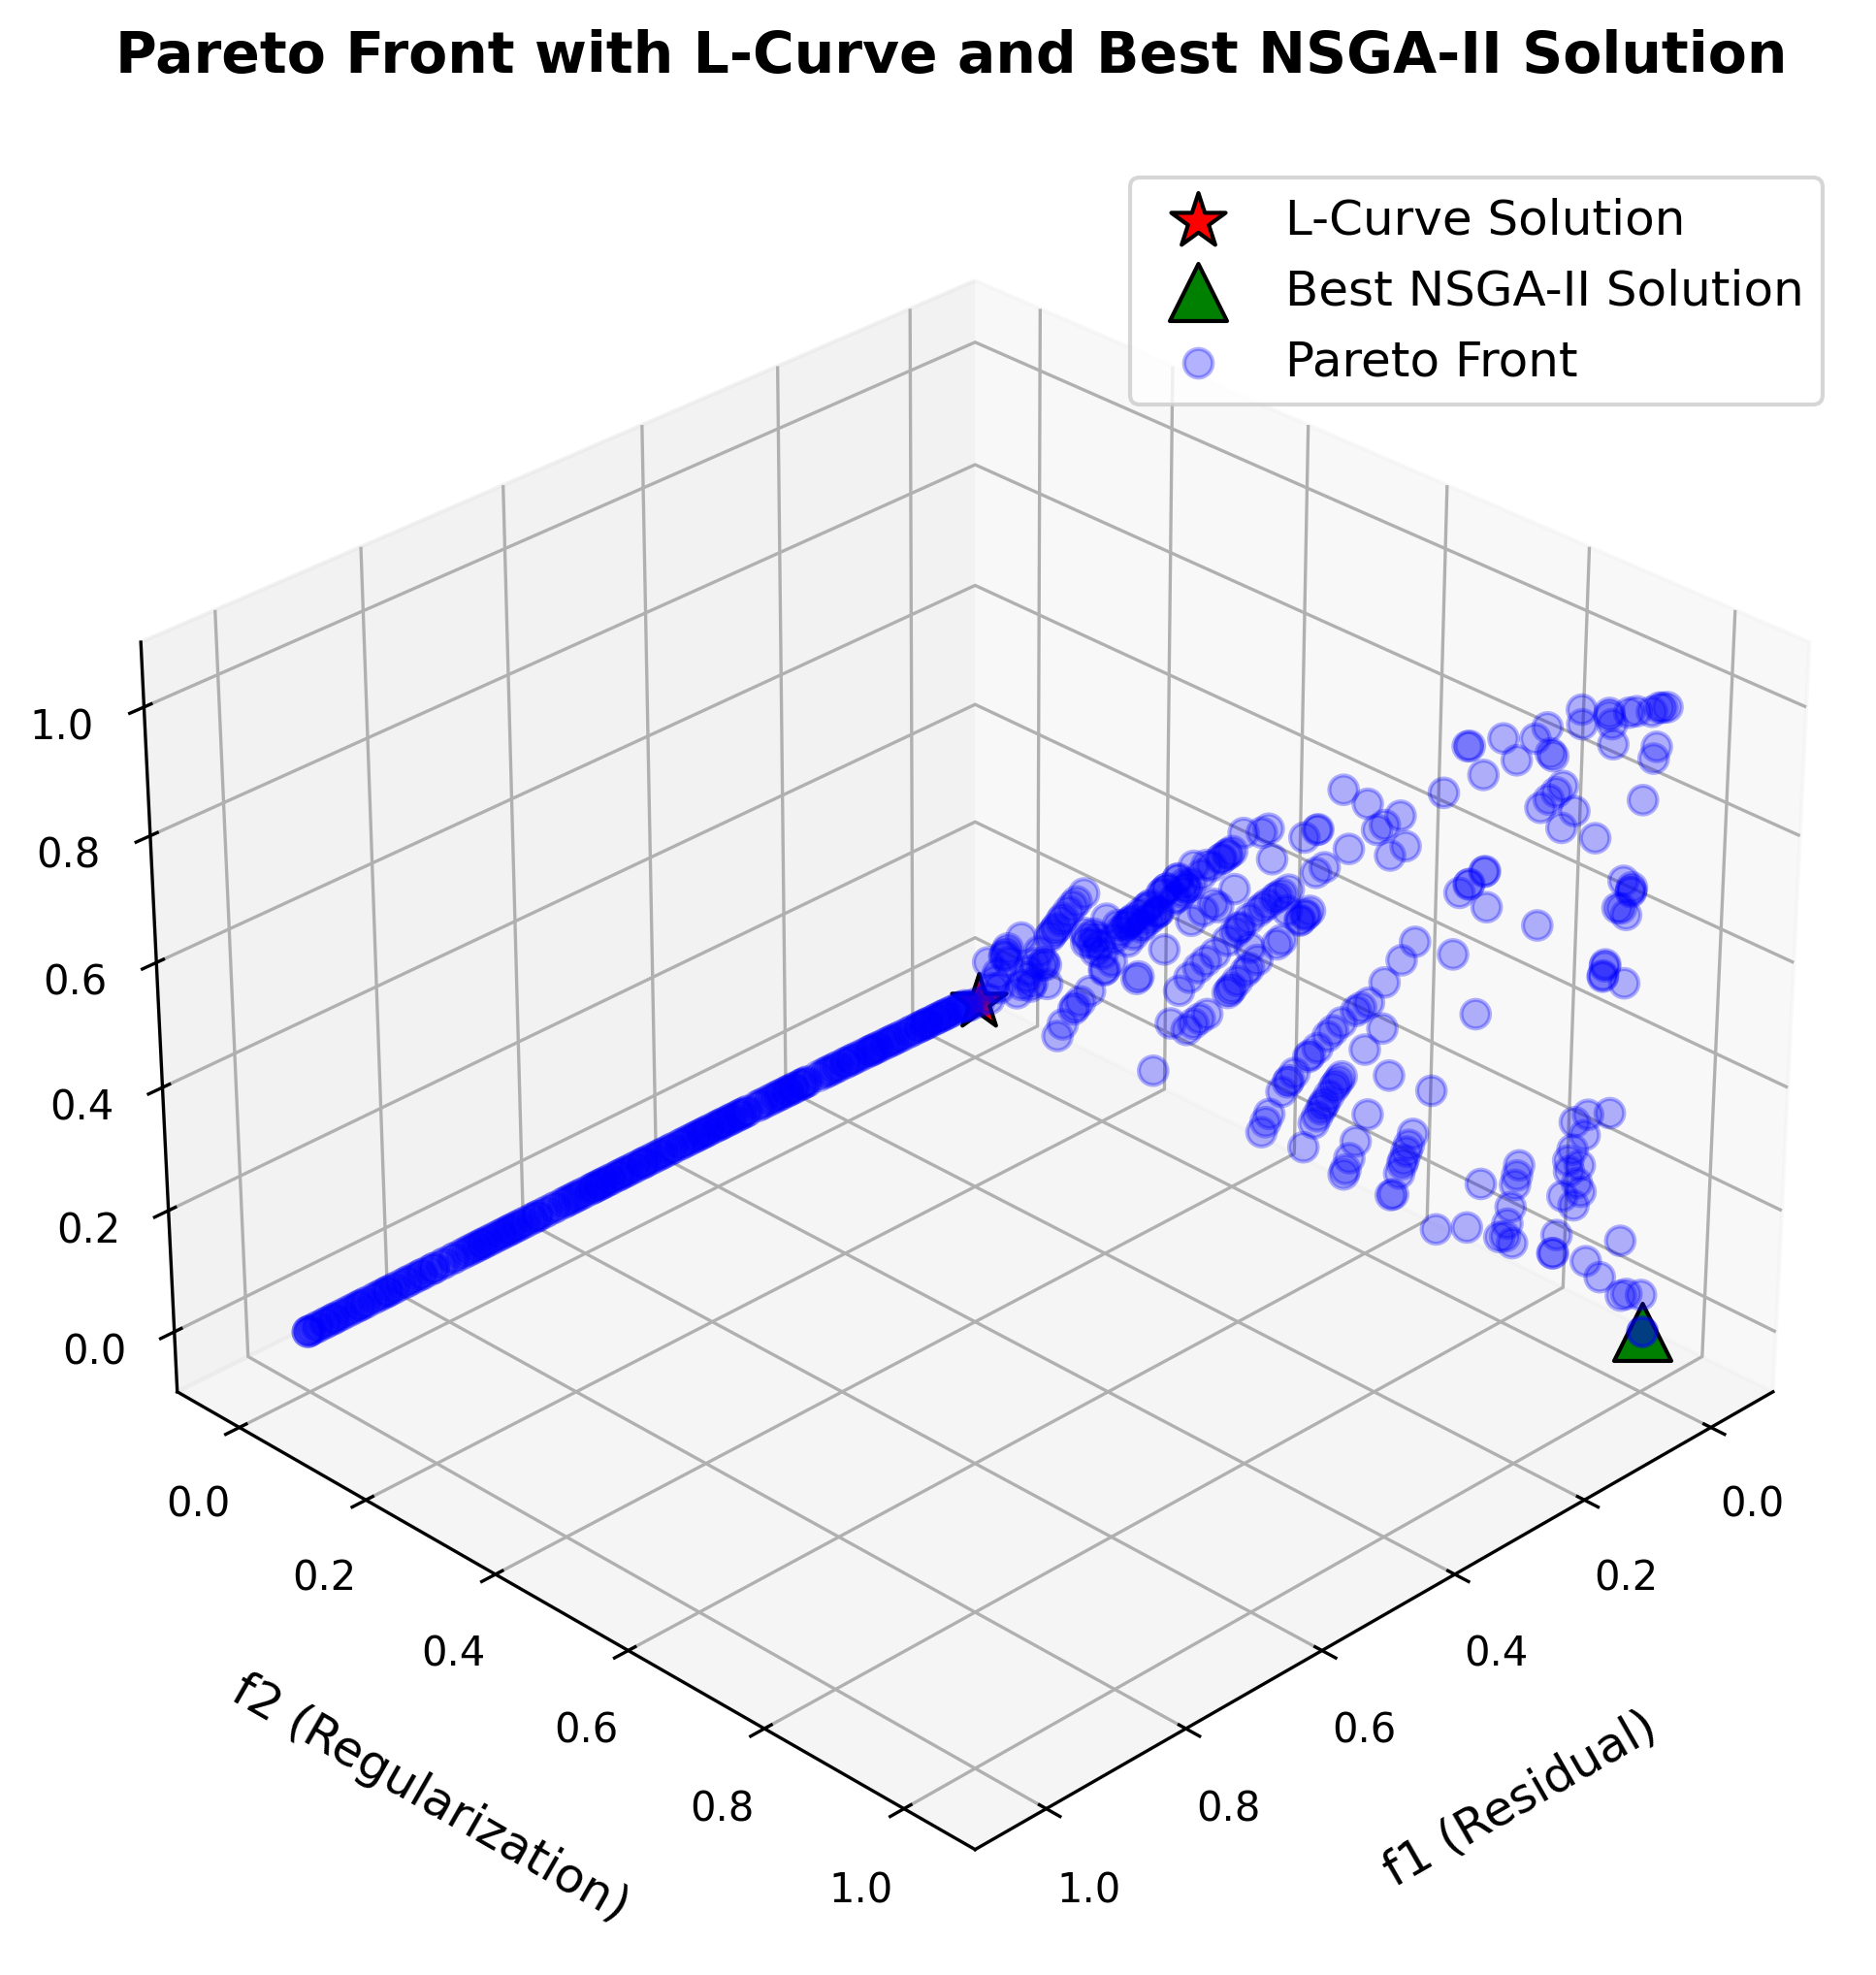
\includegraphics[width=0.8\textwidth]{Images/pareto_front_nsga2.png}
    \caption{Frente de Pareto generado por NSGA-II para \( \lambda \). Cada punto representa un compromiso entre los objetivos.}
    \label{fig:pareto_front_nsga2}
\end{figure}

\begin{figure}[H]
    \centering
    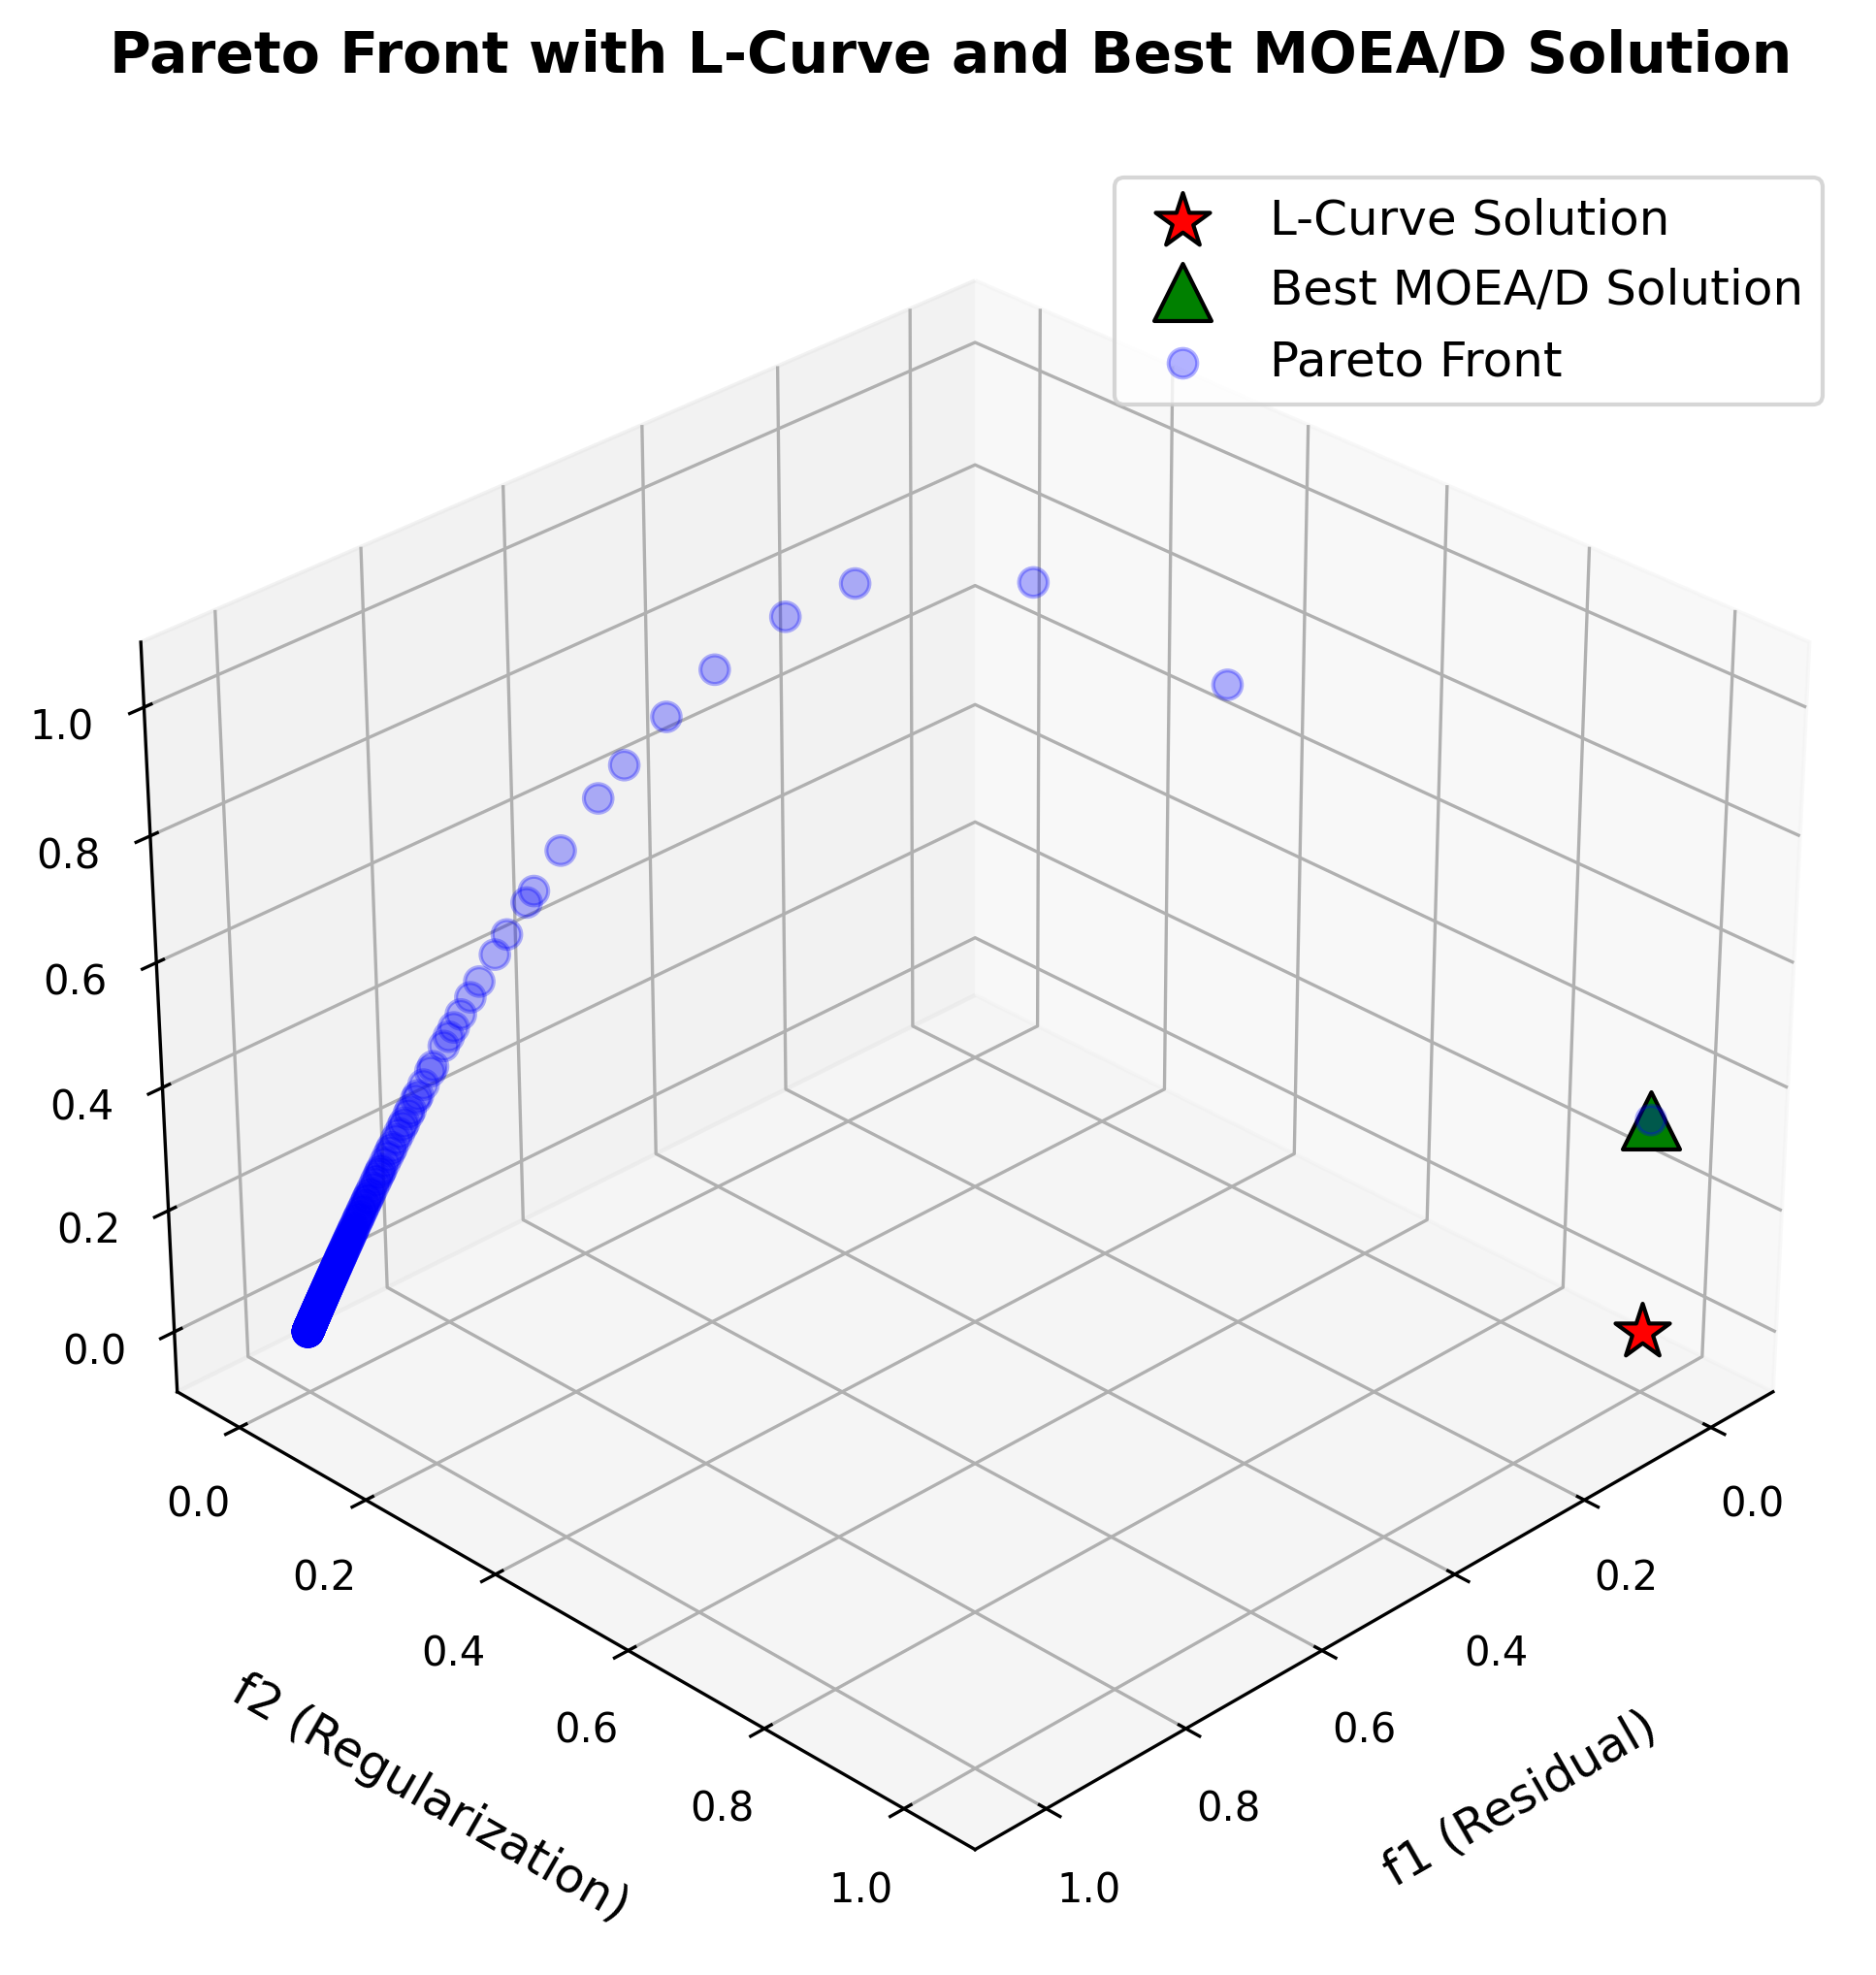
\includegraphics[width=0.8\textwidth]{Images/pareto_front_moead.png}
    \caption{Frente de Pareto generado por MOEA/D para \( \lambda \). Cada punto representa un compromiso entre los objetivos.}
    \label{fig:pareto_front_moead}
\end{figure}

Aunque ambos algoritmos exploran soluciones diversas, MOEA/D genera frentes más equilibrados debido a su enfoque basado en descomposición, mientras que NSGA-II se enfoca más en la diversidad.

\section{Análisis de Clustering de los Frentes de Pareto} \label{sec:results:clustering}

Se realizó un análisis de clustering para interpretar mejor los frentes de Pareto, identificando regiones que representan diferentes compromisos entre los objetivos. Las Figuras \ref{fig:pareto_clustering_nsga2} y \ref{fig:pareto_clustering_moead} muestran los frentes de Pareto agrupados en tres clusters para NSGA-II y MOEA/D, respectivamente.

\begin{figure}[H]
    \centering
    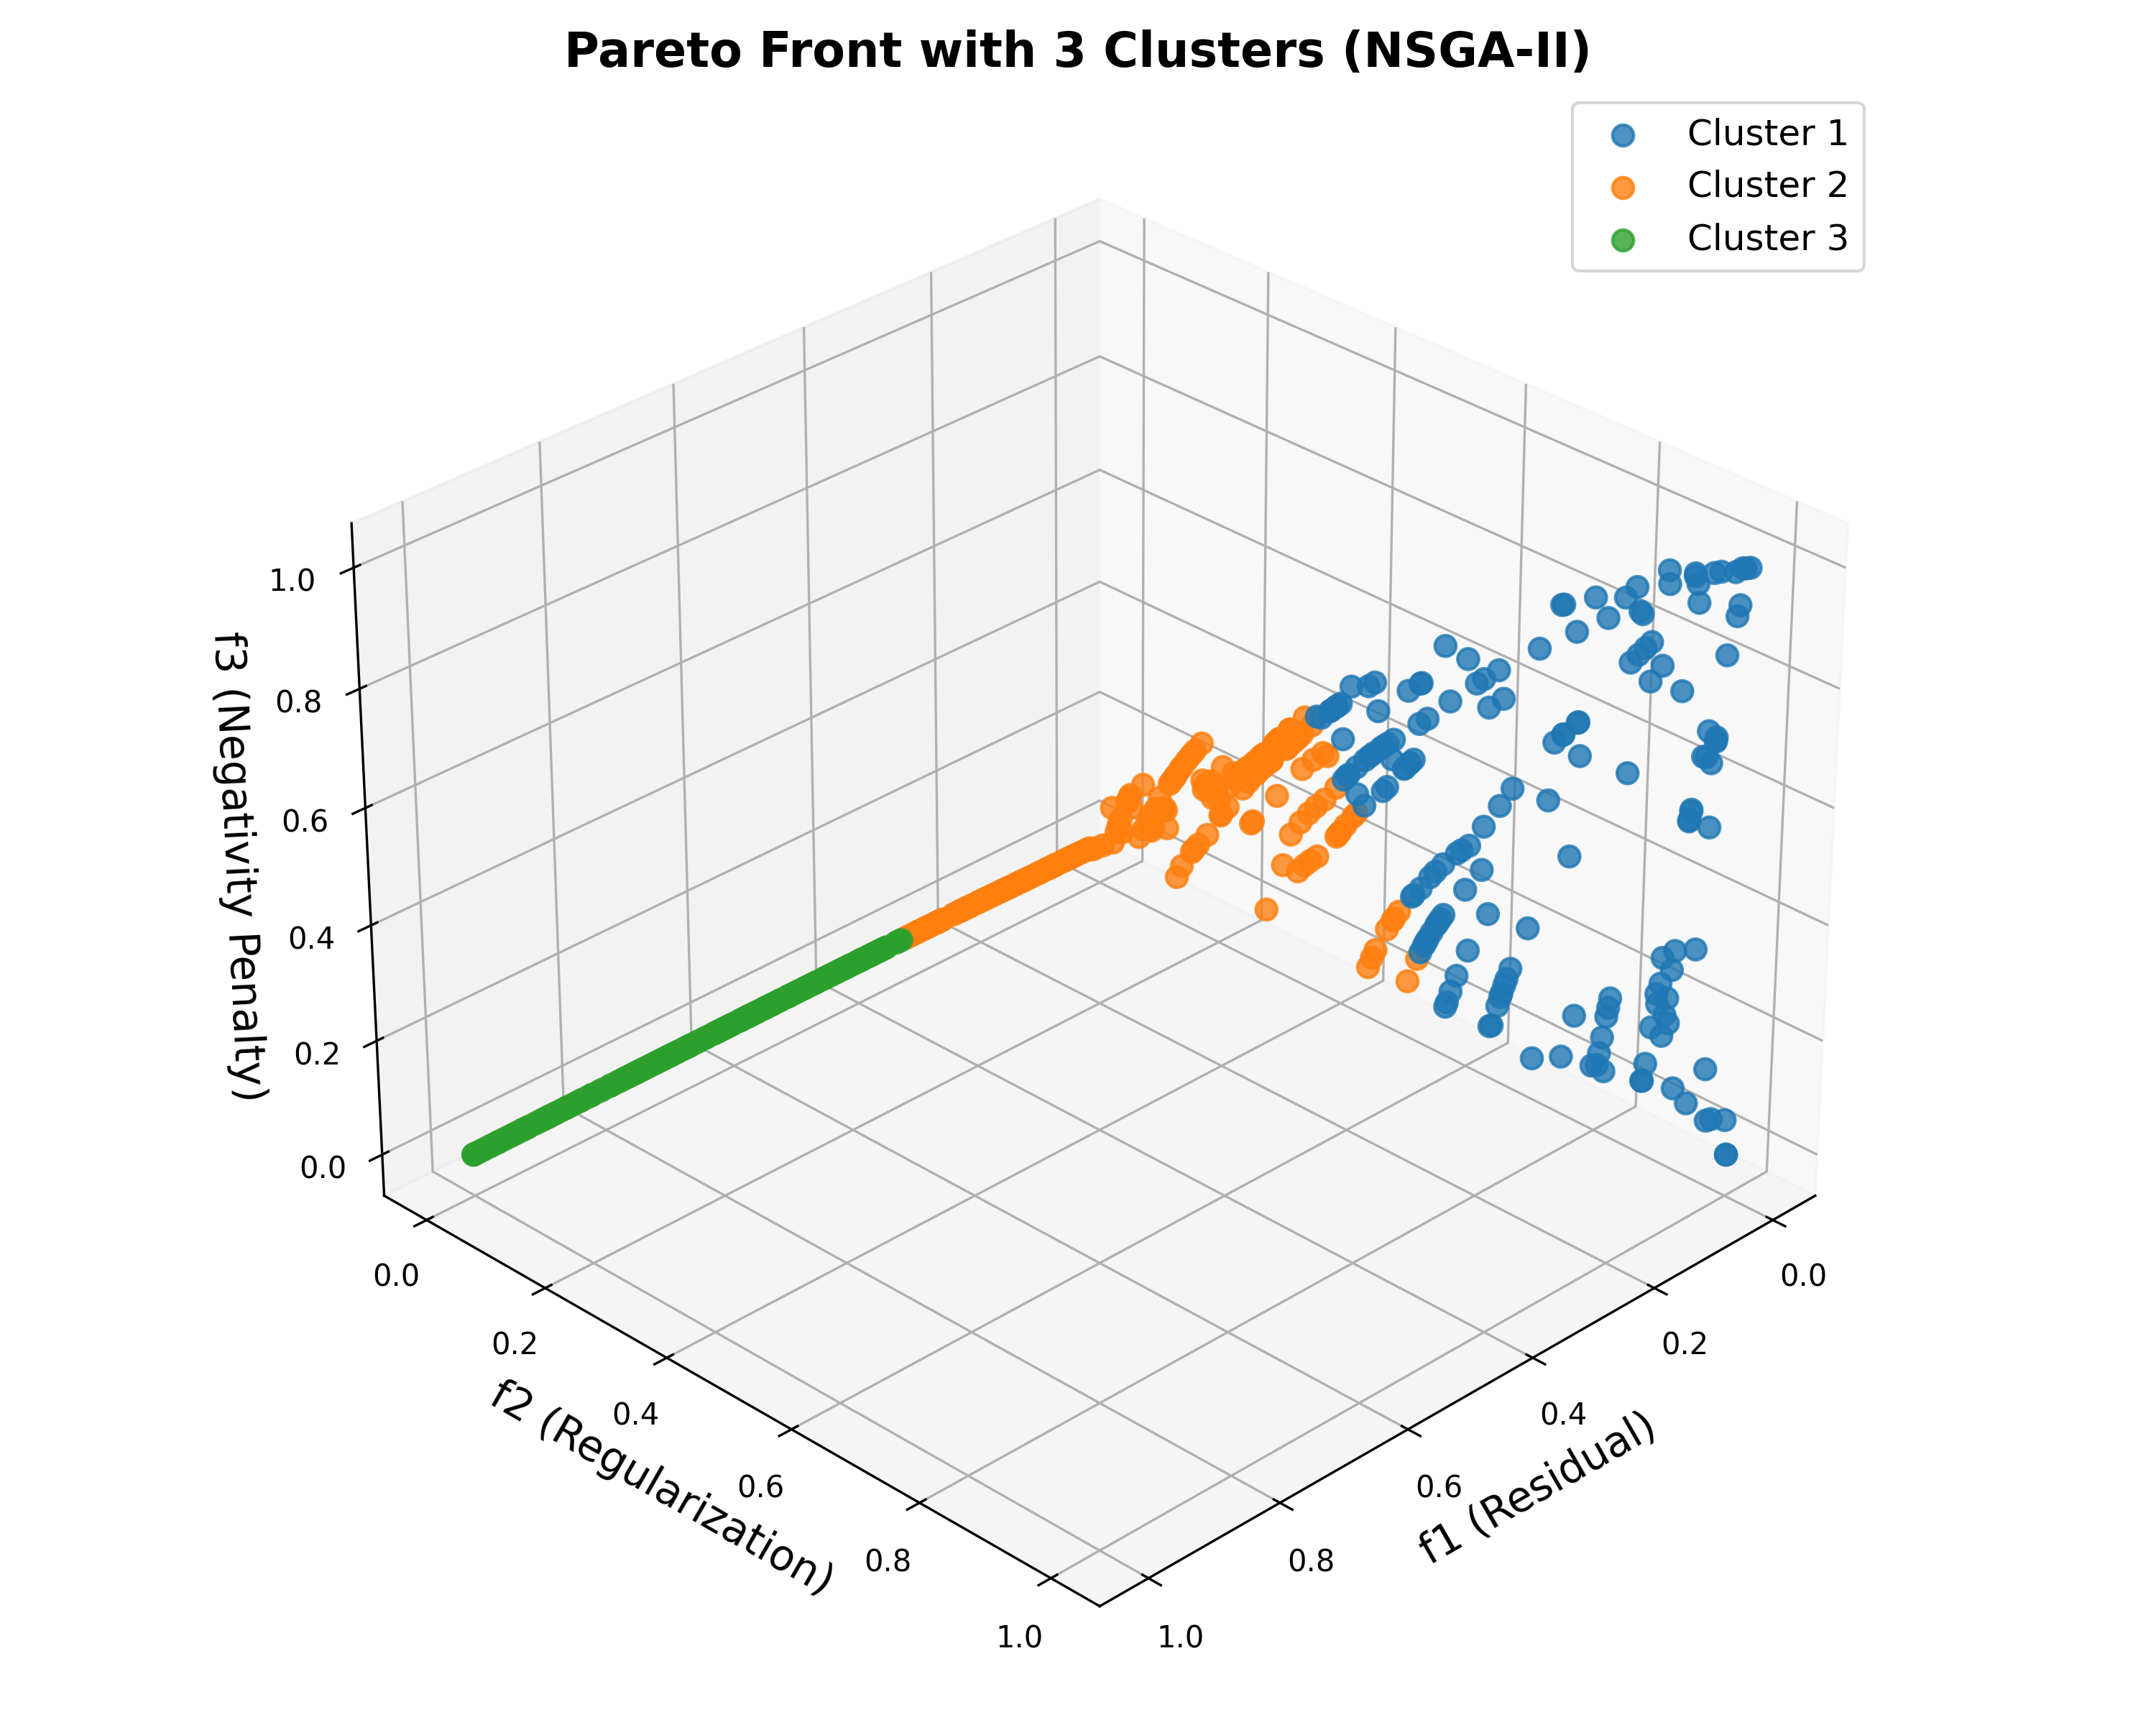
\includegraphics[width=0.8\textwidth]{Images/pareto_clustering_nsga2.png}
    \caption{Clustering del frente de Pareto generado por NSGA-II. Cada color representa un grupo de soluciones con características similares.}
    \label{fig:pareto_clustering_nsga2}
\end{figure}

\begin{figure}[H]
    \centering
    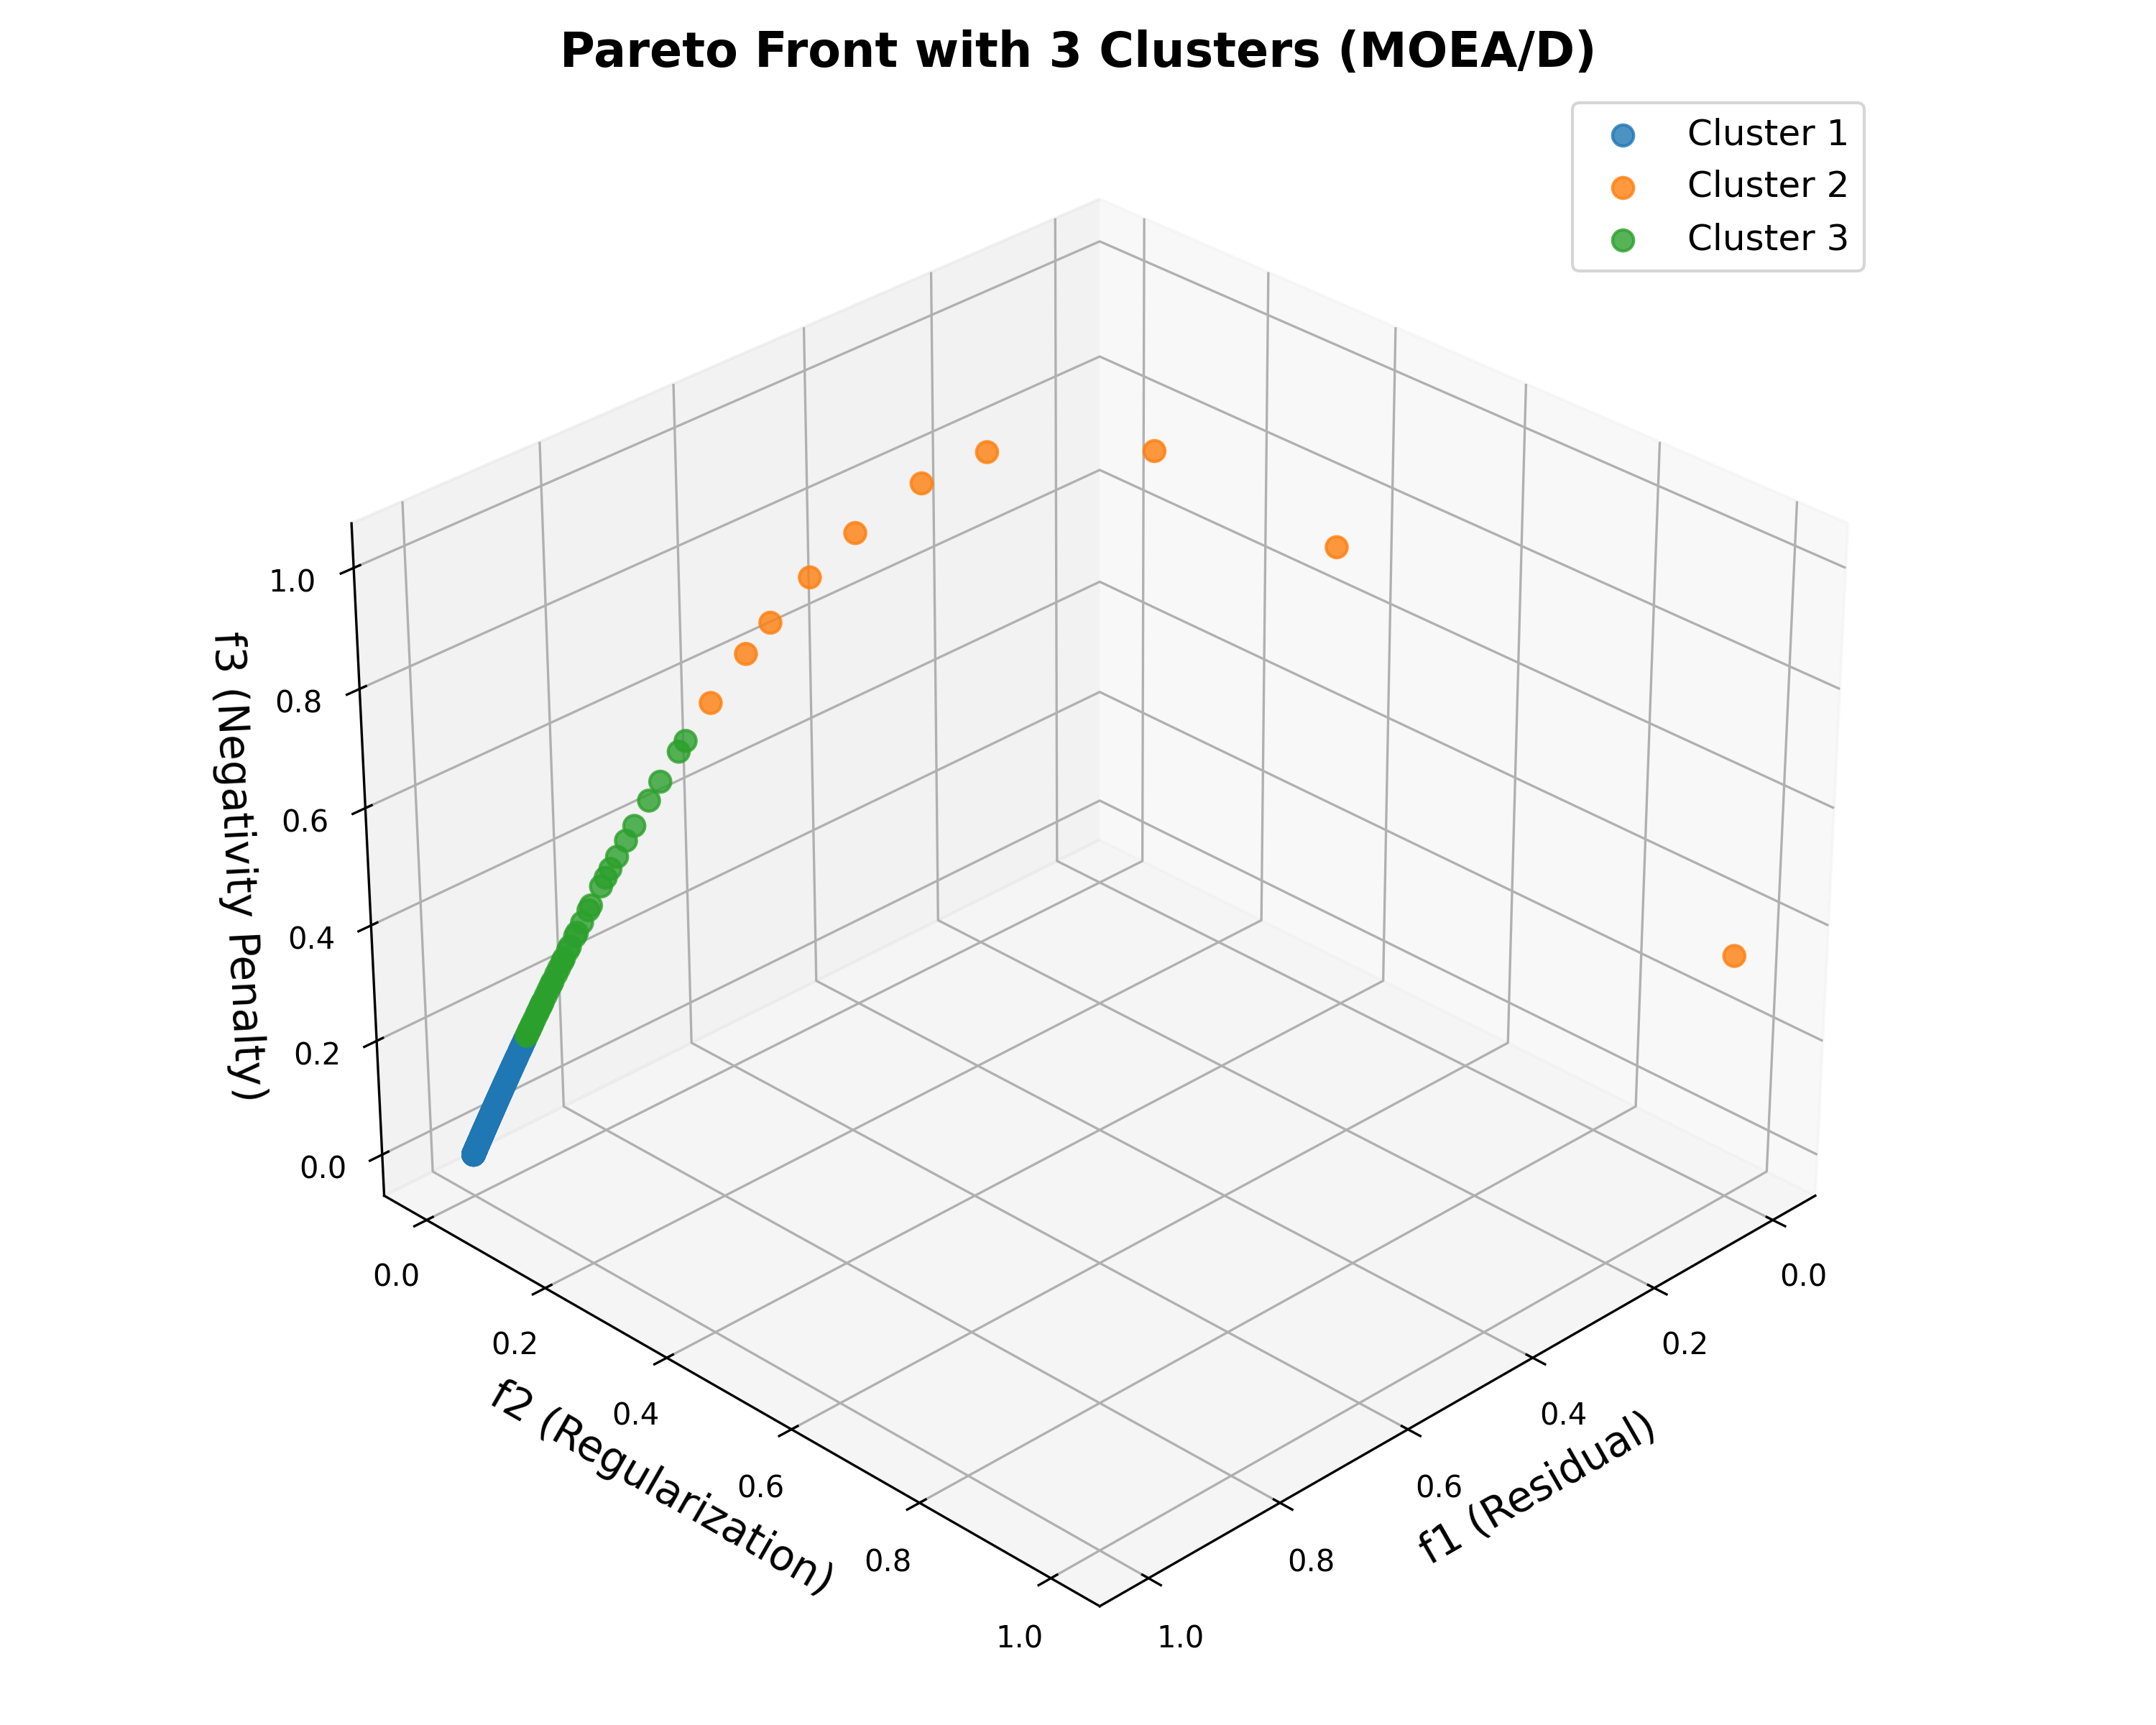
\includegraphics[width=0.8\textwidth]{Images/pareto_clustering_moead.png}
    \caption{Clustering del frente de Pareto generado por MOEA/D. Cada color representa un grupo de soluciones con características similares.}
    \label{fig:pareto_clustering_moead}
\end{figure}

El análisis revela:
\begin{itemize}
    \item NSGA-II ofrece mayor diversidad en regiones dominadas por el residual (\( f_1 \)).
    \item MOEA/D genera soluciones más uniformes en zonas con alta penalización de negatividad (\( f_3 \)).
\end{itemize}

\section{Reconstrucción del Perfil de Absorción} \label{sec:results:reconstruction}

Las Figuras \ref{fig:reconstruction_profiles_nsga2} y \ref{fig:reconstruction_profiles_moead} presentan los perfiles de absorción \( \mathbf{\mu} \) reconstruidos utilizando los valores de \( \lambda \) obtenidos con NSGA-II y MOEA/D para \( \sigma^2 = 10^{-1} \), respectivamente.

\begin{figure}[H]
    \centering
    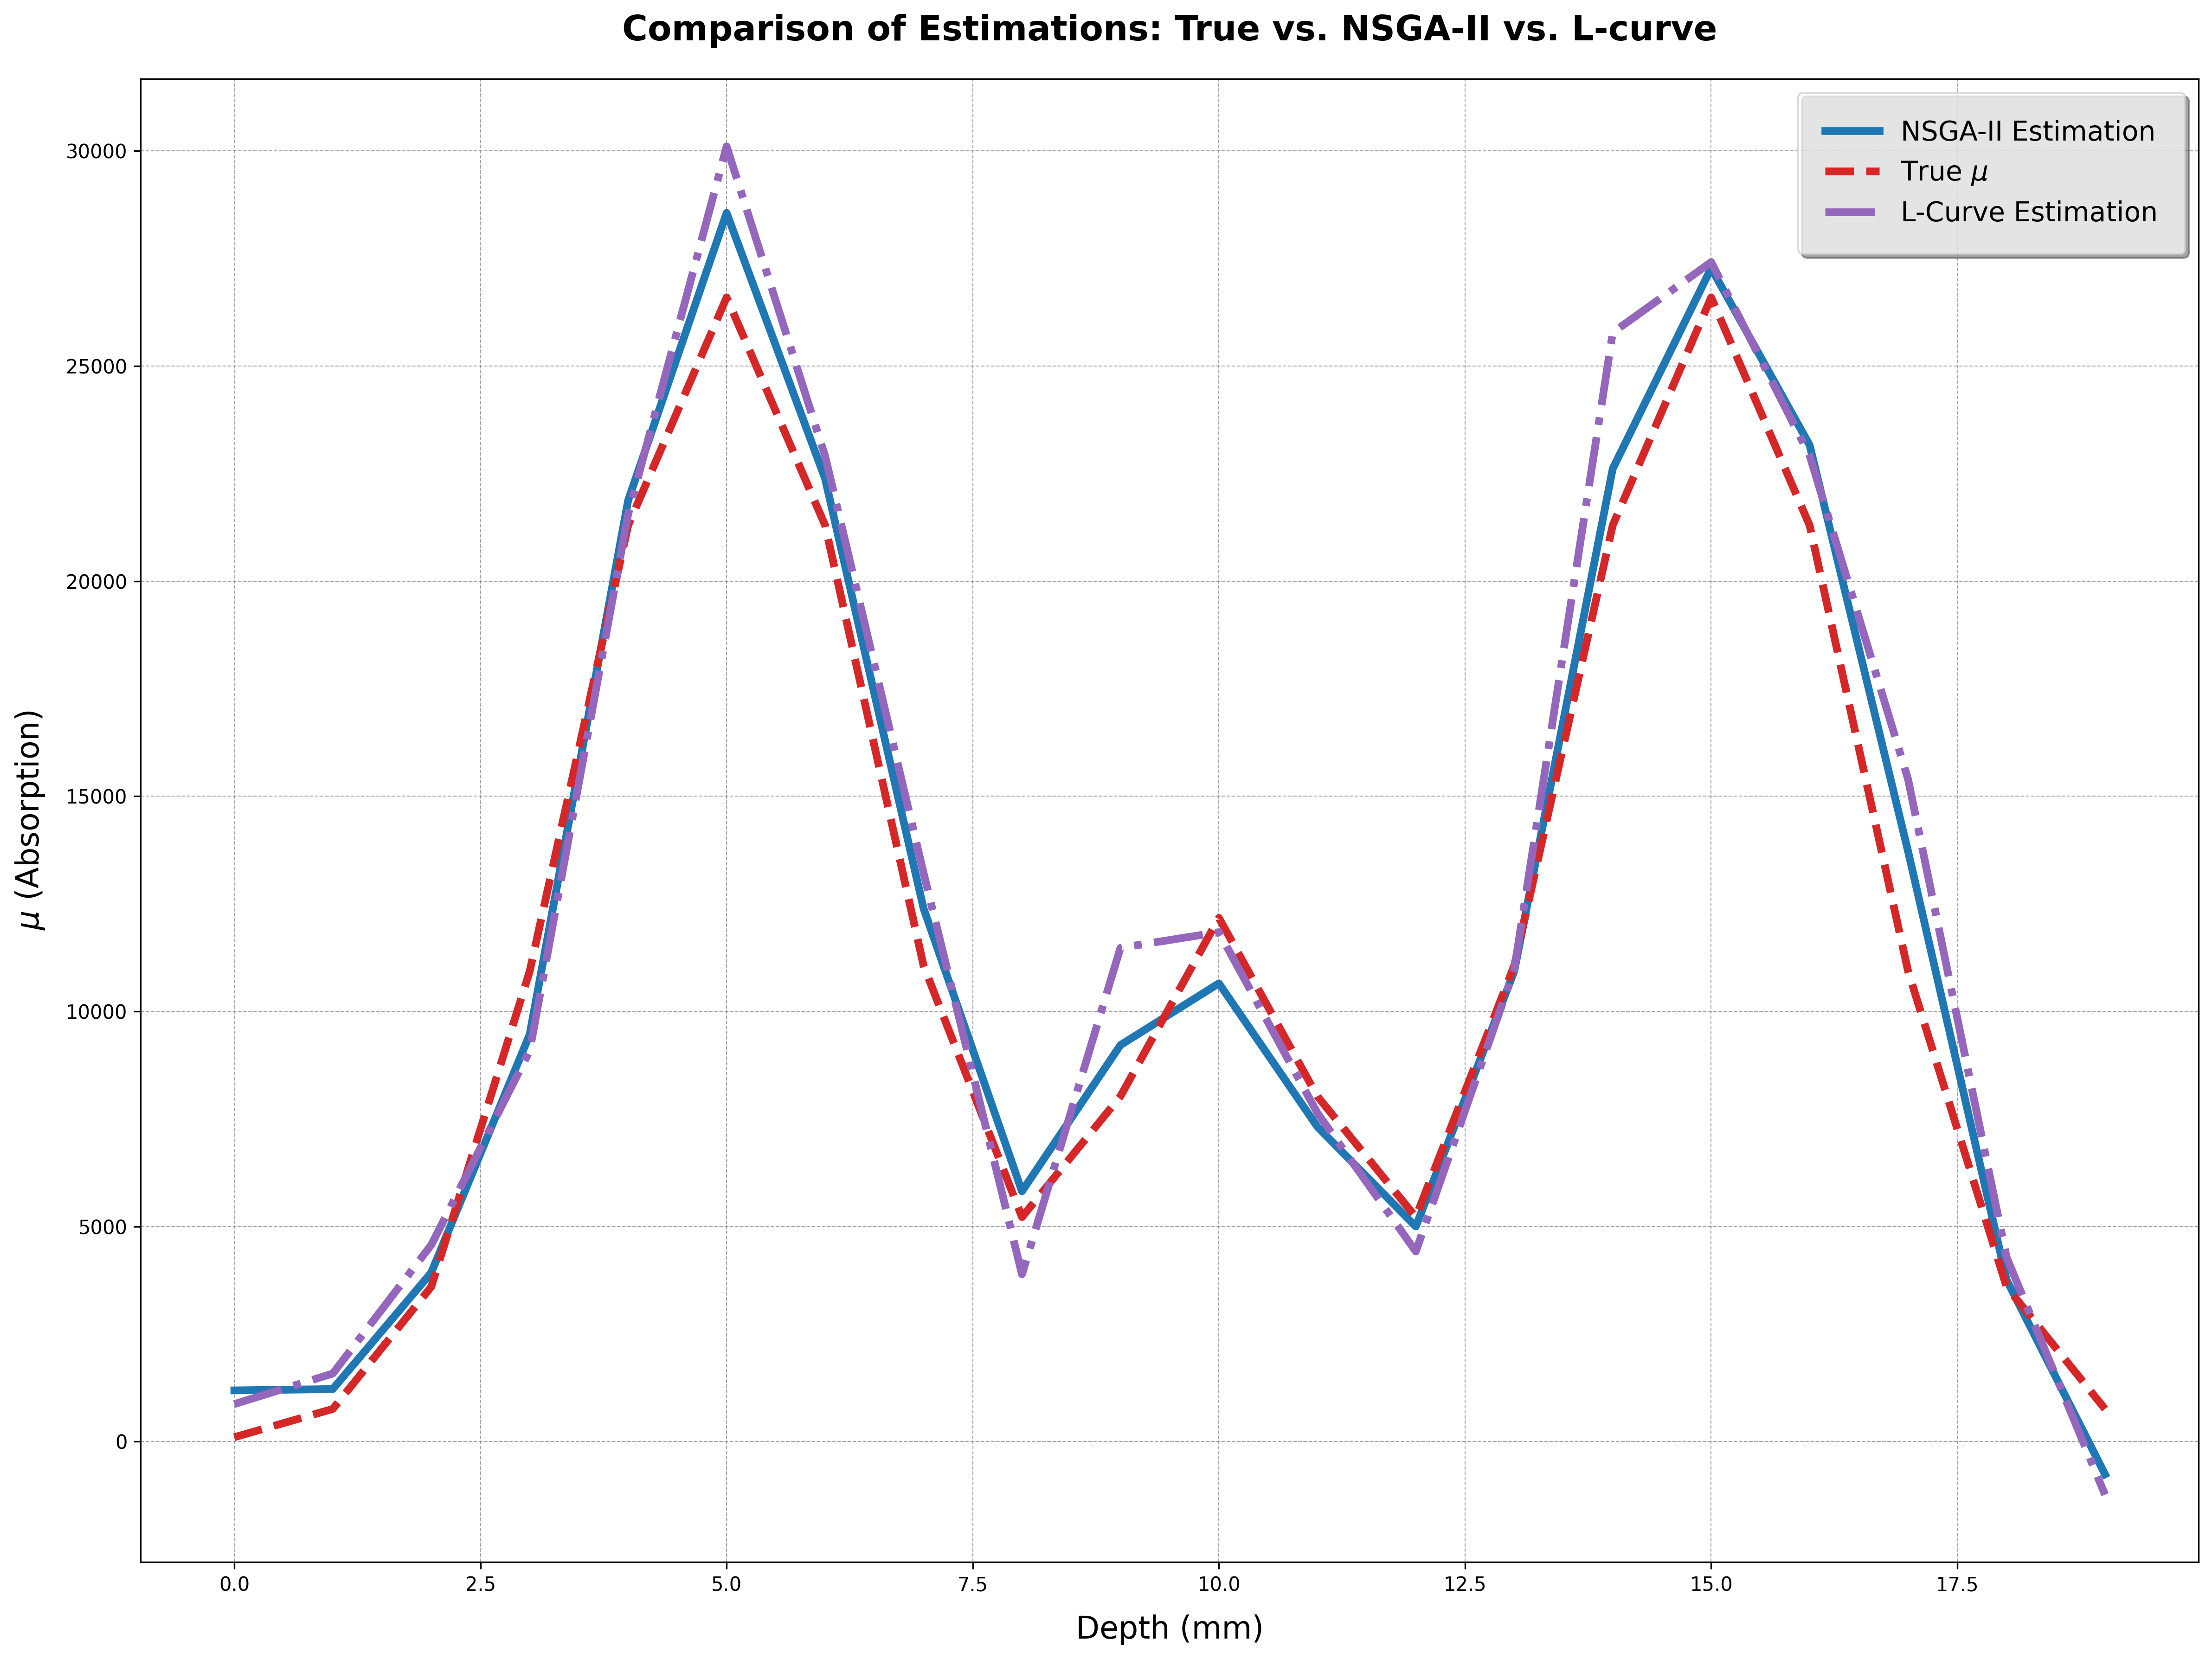
\includegraphics[width=0.8\textwidth]{Images/reconstruction_profiles_nsga2.png}
    \caption{Perfiles de absorción reconstruidos utilizando NSGA-II. La curva azul representa el perfil real y la curva roja corresponde a la solución reconstruida.}
    \label{fig:reconstruction_profiles_nsga2}
\end{figure}

\begin{figure}[H]
    \centering
    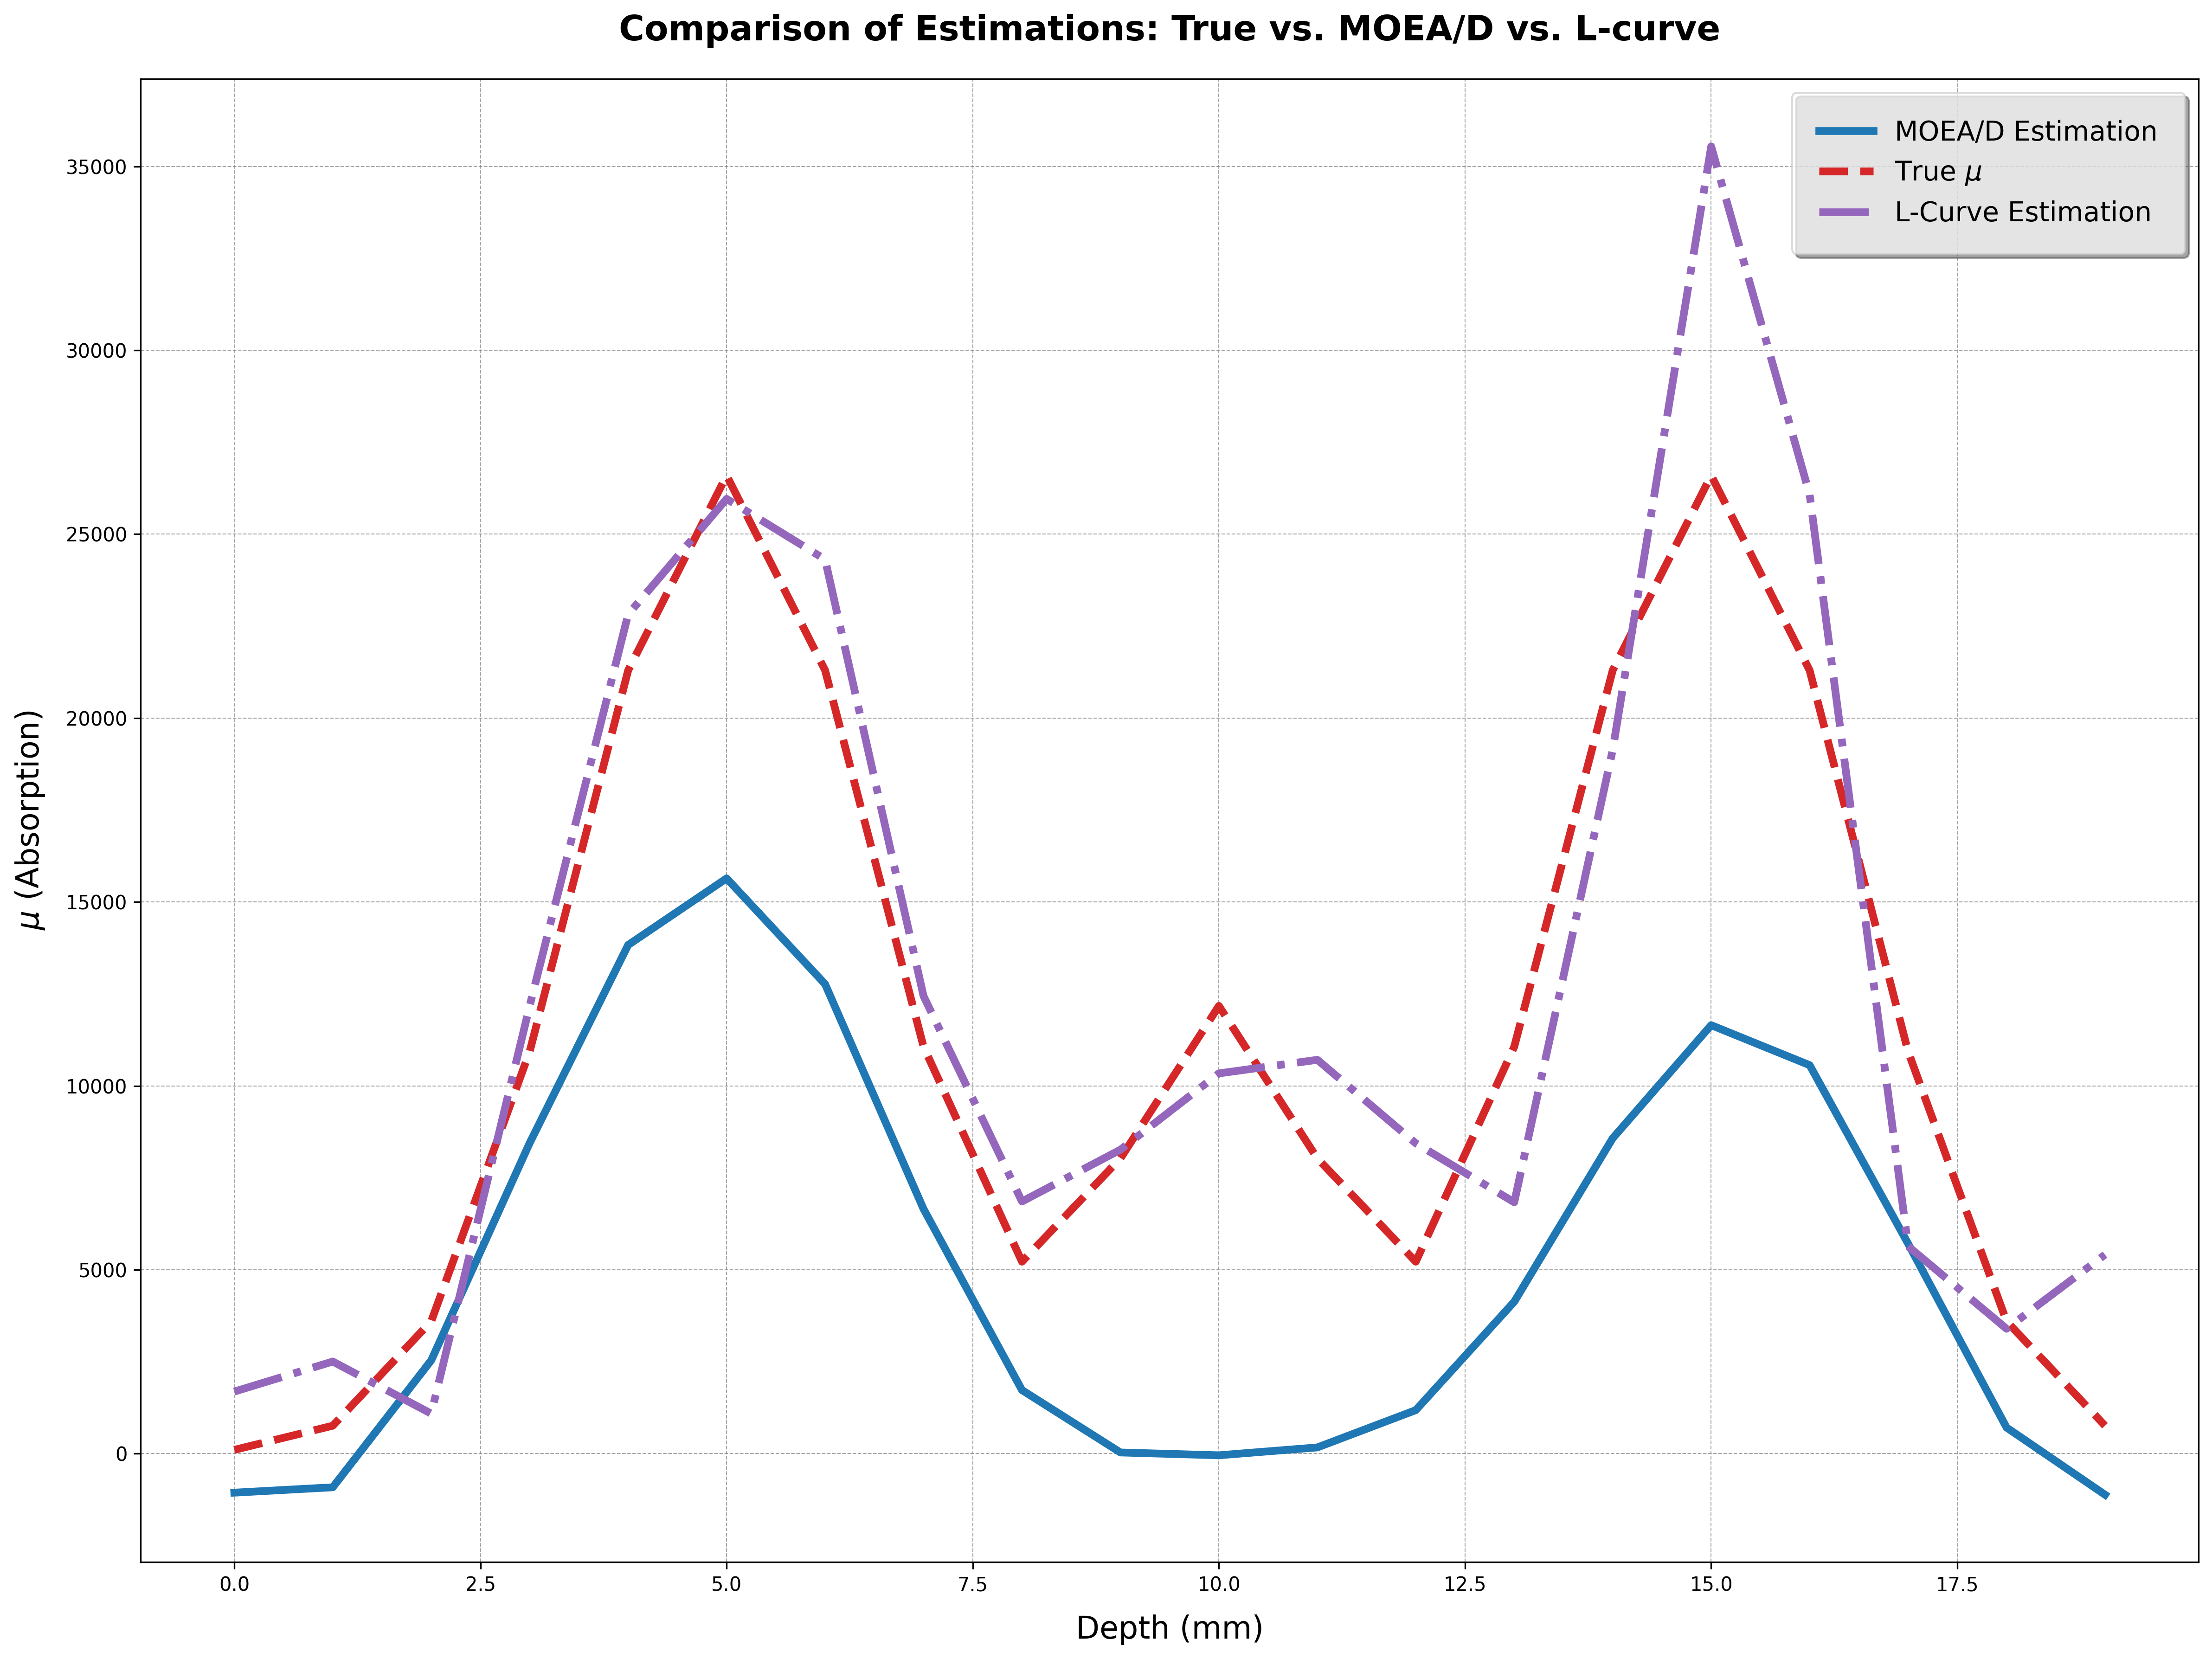
\includegraphics[width=0.8\textwidth]{Images/reconstruction_profiles_moead.png}
    \caption{Perfiles de absorción reconstruidos utilizando MOEA/D. La curva azul representa el perfil real y la curva verde corresponde a la solución reconstruida.}
    \label{fig:reconstruction_profiles_moead}
\end{figure}

Ambos métodos producen reconstrucciones físicamente consistentes en comparación con el método de la curva L, pero MOEA/D genera perfiles más estables en condiciones de ruido elevado.

\section{Comparación entre NSGA-II, MOEA/D y la Curva L} \label{sec:results:comparison}

En esta sección se evalúan las soluciones obtenidas mediante NSGA-II, MOEA/D y la solución propuesta por la curva L. La Tabla \ref{tab:comparison_algorithms} resume los valores de los objetivos normalizados para cada metodología para \( \sigma^2 = 10^{-1} \).

\begin{table}[h]
    \centering
    \begin{tabular}{lccc}
        \toprule
        \textbf{Método} & \textbf{Fidelidad (\( f_1 \))} & \textbf{Regularización (\( f_2 \))} & \textbf{Negatividad (\( f_3 \))} \\
        \midrule
        NSGA-II (mejor solución) & 0.000 & 1.000 & 0.000 \\
        MOEA/D (mejor solución) & 0.000 & 1.000 & 0.347 \\
        Curva L & 0.00063 & 0.0071 & 0.0001 \\
        \bottomrule
    \end{tabular}
    \caption{Comparación de las métricas entre NSGA-II, MOEA/D y la curva L. Los valores están normalizados para permitir una evaluación directa.}
    \label{tab:comparison_algorithms}
\end{table}

\noindent
\textbf{Observaciones:}
\begin{itemize}
    \item \textbf{NSGA-II:} Este algoritmo generó la solución con los mejores valores de fidelidad (\( f_1 \)) y negatividad (\( f_3 \)), destacándose en situaciones donde la prioridad es maximizar la precisión y garantizar la consistencia física de la solución.
    \item \textbf{MOEA/D:} Aunque alcanzó valores similares en fidelidad (\( f_1 \)) y regularización (\( f_2 \)) en comparación con NSGA-II, este algoritmo ofreció soluciones con un balance más equitativo entre los tres objetivos, lo que puede ser beneficioso en aplicaciones donde la penalización de la negatividad (\( f_3 \)) no sea tan estricta.
    \item \textbf{Curva L:} Este enfoque tradicional produjo soluciones menos competitivas en todos los objetivos, ya que se centra únicamente en encontrar un compromiso entre fidelidad y regularización, sin considerar objetivos adicionales como la penalización de valores negativos. Sin embargo, destaca por su simplicidad y bajo costo computacional.
\end{itemize}

La selección de las "mejores" soluciones se realizó utilizando un sistema de puntuación ponderado, donde se asignó mayor importancia a la fidelidad (\( f_1 \)) y la regularización (\( f_2 \)), mientras que se aplicó una penalización significativa a la negatividad (\( f_3 \)). Las ponderaciones utilizadas fueron \([0.6, 0.1, 0.3]\), reflejando la prioridad otorgada a cada objetivo en el análisis.

% \noindent
% \textbf{Análisis Comparativo:}

% NSGA-II y MOEA/D muestran una ventaja significativa frente a la curva L al permitir una exploración más amplia y detallada de los compromisos entre objetivos. MOEA/D se distingue por su capacidad para equilibrar objetivos, mientras que NSGA-II es ideal para priorizar fidelidad y minimizar negatividad. Por otro lado, la curva L sigue siendo útil como referencia inicial debido a su simplicidad, aunque carece de la flexibilidad y adaptabilidad que ofrecen los algoritmos evolutivos.

% Estos resultados subrayan la importancia de elegir el enfoque de optimización según los requisitos específicos del problema. En aplicaciones donde la calidad física de las soluciones y el manejo de restricciones son prioritarios, NSGA-II y MOEA/D son opciones superiores, mientras que la curva L podría ser más adecuada para configuraciones iniciales o en problemas menos complejos.

\section{Impacto del Ruido en el RMSE} \label{sec:results:noise}

Las Figuras \ref{fig:rmse_nsga2} y \ref{fig:rmse_moead} muestran el RMSE promedio obtenido para diferentes niveles de varianza del ruido (\( \sigma^2 \)) utilizando NSGA-II y MOEA/D, respectivamente.

\begin{figure}[H]
    \centering
    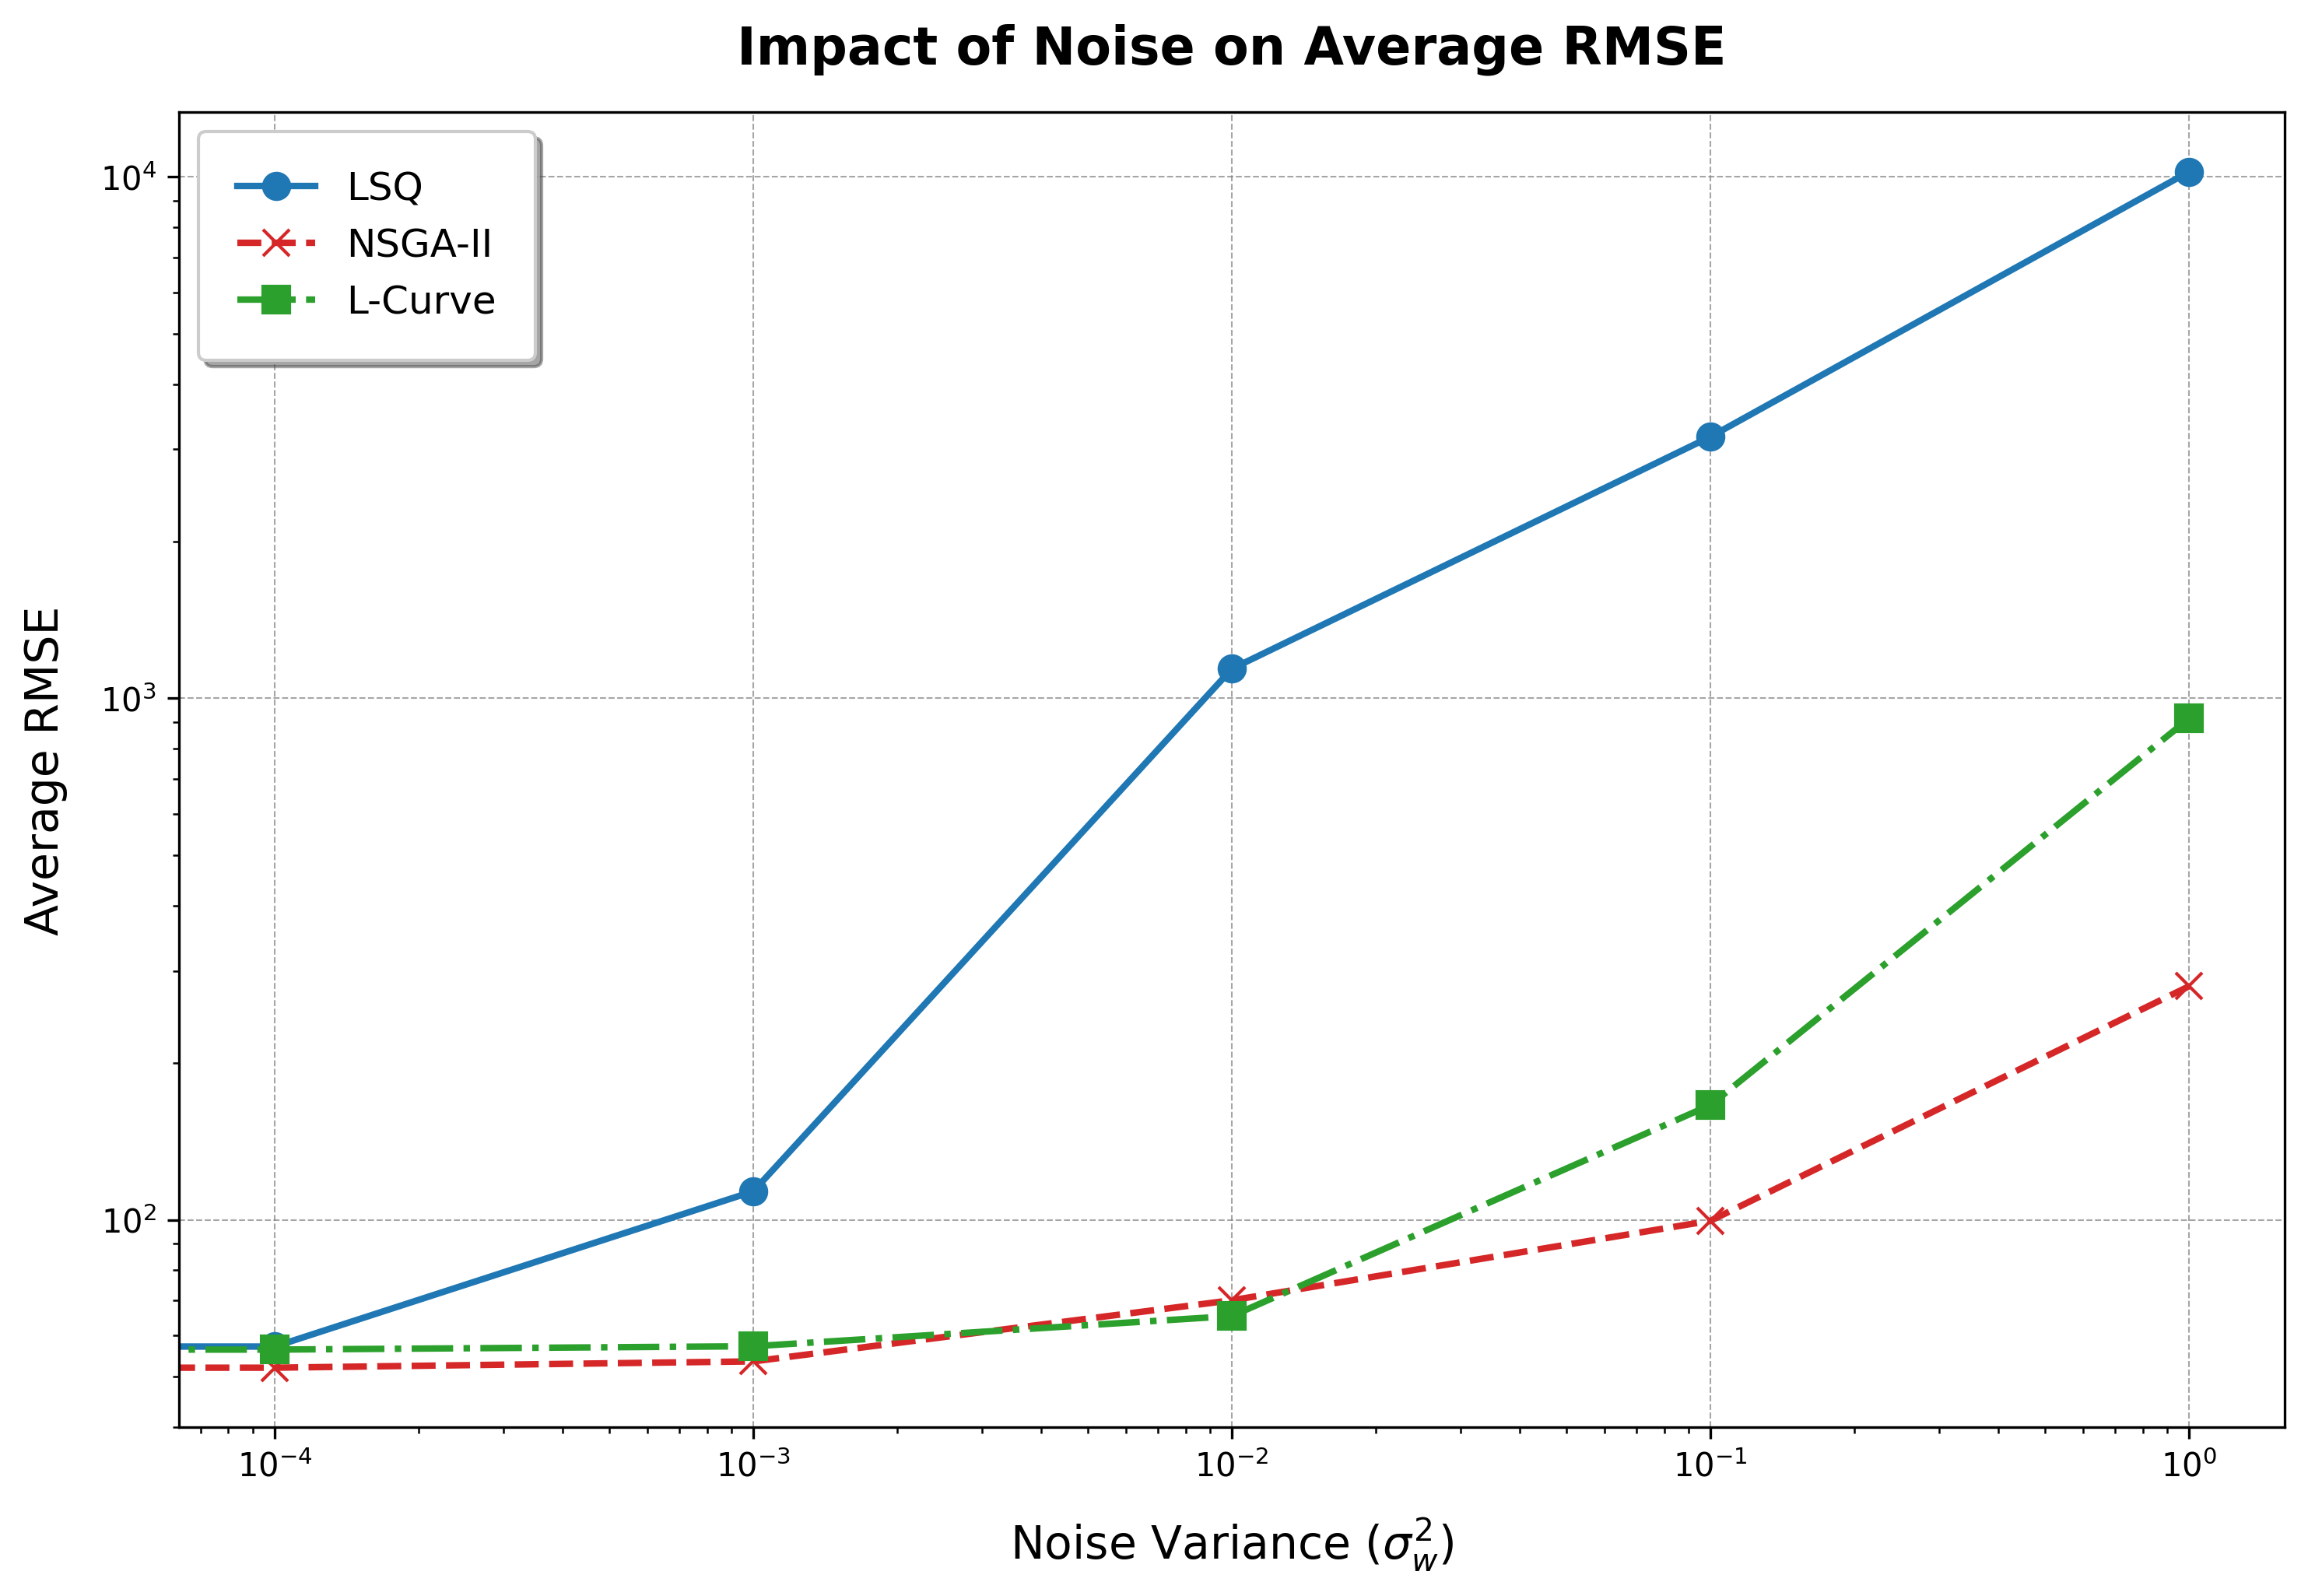
\includegraphics[width=0.8\textwidth]{Images/impact_noise_on_rmse_nsga2.png}
    \caption{Impacto del ruido en el RMSE promedio utilizando NSGA-II para diferentes valores de \( \sigma^2 \).}
    \label{fig:rmse_nsga2}
\end{figure}

\begin{figure}[H]
    \centering
    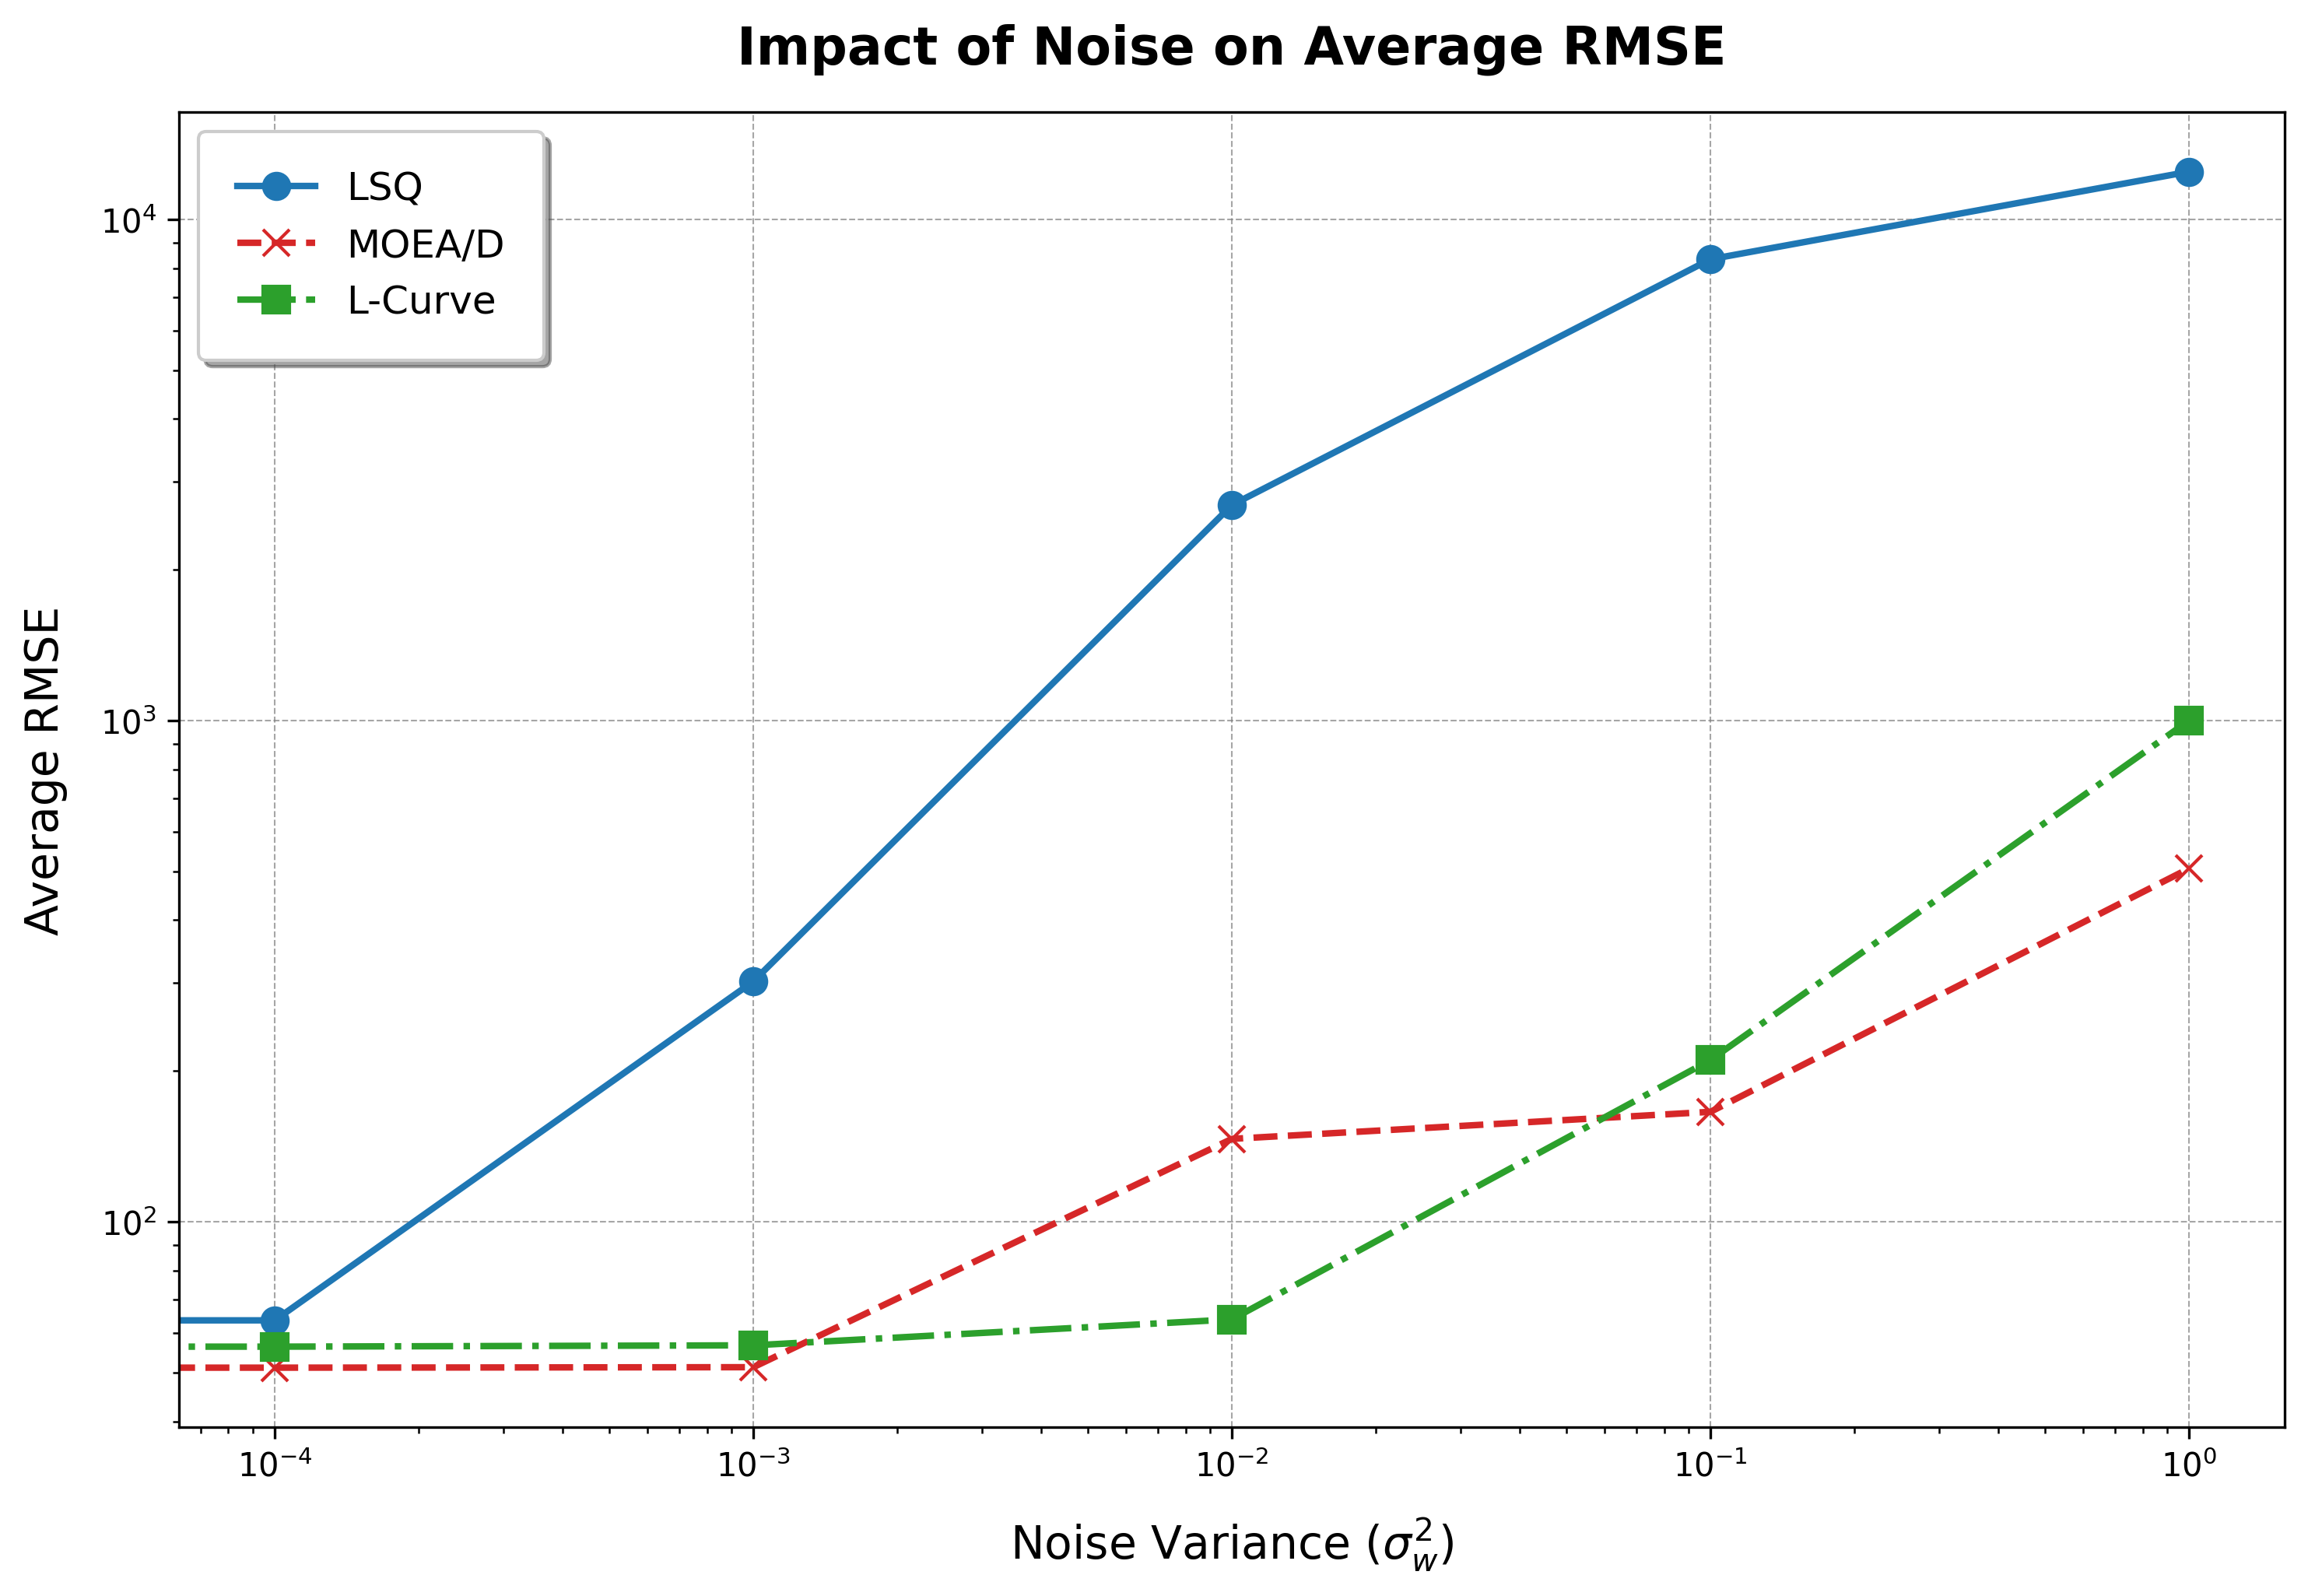
\includegraphics[width=0.8\textwidth]{Images/impact_noise_on_rmse_moead.png}
    \caption{Impacto del ruido en el RMSE promedio utilizando MOEA/D para diferentes valores de \( \sigma^2 \).}
    \label{fig:rmse_moead}
\end{figure}

Observaciones clave:
\begin{itemize}
    \item NSGA-II mantiene un RMSE más estable incluso en niveles altos de ruido, demostrando mejor adaptabilidad en condiciones adversas.
    \item MOEA/D es robusto a niveles bajos y moderados de ruido, pero muestra mayor sensibilidad para \( \sigma^2 > 10^{-1} \).
\end{itemize}


\section{Correlaciones entre Objetivos y Proyecciones en 2D} \label{sec:results:correlation}

Para interpretar mejor los compromisos entre los objetivos definidos (\(f_1\), \(f_2\), \(f_3\)), se analizaron las correlaciones entre ellos y se visualizaron las proyecciones en 2D de los frentes de Pareto generados por NSGA-II y MOEA/D.

\subsubsection{Correlaciones entre Objetivos}

La Figura \ref{fig:correlation_matrix} presenta la matriz de correlación entre las funciones objetivo \( f_1 \) (residual), \( f_2 \) (regularización) y \( f_3 \) (penalización de valores negativos), calculada utilizando las soluciones del frente de Pareto generado por MOEA/D y NSGA-II para \( \sigma^2 = 10^{-1} \).

\begin{figure}[H]
    \centering
    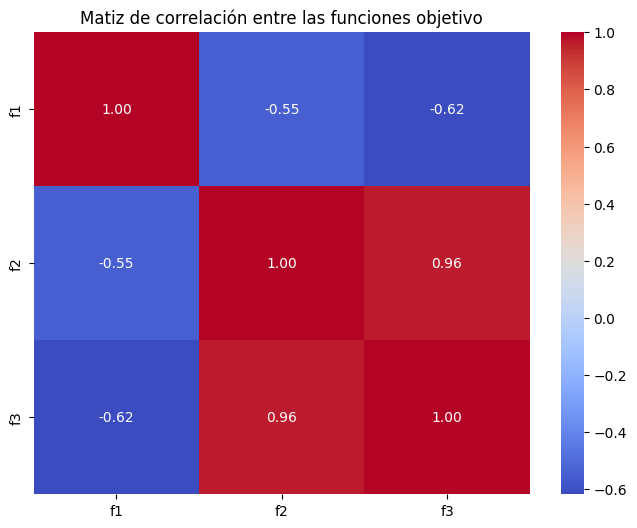
\includegraphics[width=0.7\textwidth]{Images/correlation_matrix.png}
    \caption{Matriz de correlación entre las funciones objetivo \( f_1 \), \( f_2 \), y \( f_3 \).}
    \label{fig:correlation_matrix}
\end{figure}

Los resultados destacan las siguientes tendencias clave:
\begin{itemize}
    \item Existe una correlación negativa entre \( f_1 \) y \( f_3 \) (\(-0.62\)) y entre \( f_1 \) y \( f_2 \) (\(-0.55\)), lo que refleja un compromiso entre minimizar el residual y garantizar soluciones físicamente consistentes.
    \item Se observa una alta correlación positiva entre \( f_2 \) y \( f_3 \) (\(0.96\)), lo que sugiere que aumentar la regularización también promueve soluciones con menor penalización por valores negativos.
    \item Estos patrones indican que los objetivos no son completamente independientes, y los algoritmos deben gestionar cuidadosamente estas correlaciones al explorar el espacio de soluciones.
\end{itemize}

Este análisis permite identificar relaciones entre objetivos, lo que facilita priorizar soluciones específicas según las necesidades de la aplicación.

\section{Proyecciones en 2D de los Objetivos}

\subsection{Proyecciones en 2D de los Objetivos (NSGA-II)}

Para analizar las relaciones entre los objetivos definidos, se realizaron proyecciones bidimensionales de las soluciones obtenidas con NSGA-II en el frente de Pareto. La Figura \ref{fig:objective_projections_nsga2} muestra las distribuciones marginales de cada objetivo (\(f_1\), \(f_2\) y \(f_3\)) en las diagonales principales, y los diagramas de dispersión para cada par de objetivos en las subgráficas restantes.

\begin{figure}[H]
    \centering
    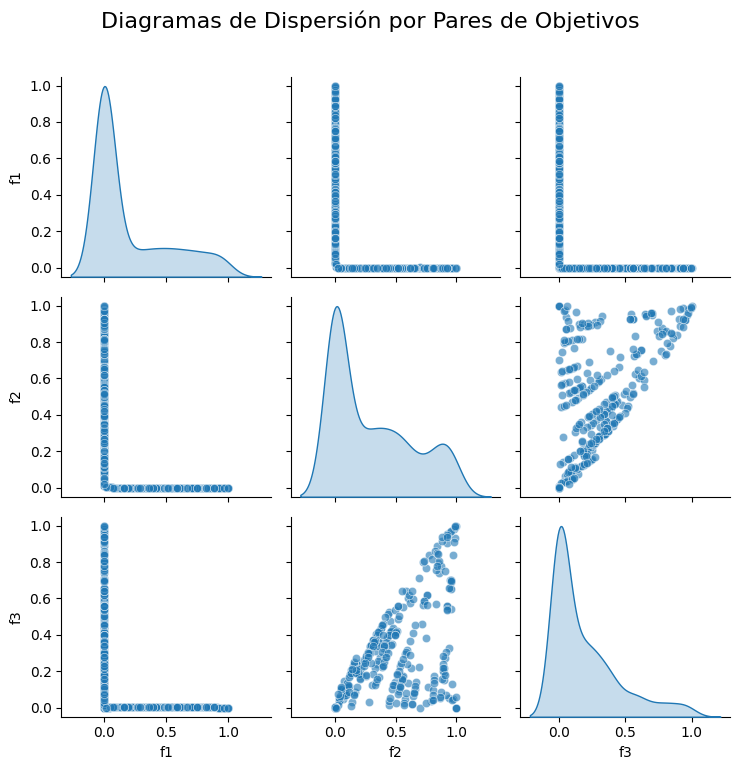
\includegraphics[width=0.9\textwidth]{Images/pareto_projection_nsga2.png}
    \caption{Proyecciones en 2D entre los objetivos \( f_1 \), \( f_2 \) y \( f_3 \) para NSGA-II. Cada subgráfica representa la relación entre dos objetivos, mientras que las distribuciones marginales se encuentran en la diagonal.}
    \label{fig:objective_projections_nsga2}
\end{figure}

\textbf{Observaciones clave:}
\begin{itemize}
    \item La relación entre \(f_2\) (regularización) y \(f_3\) (penalización de negatividad) es aproximadamente lineal, lo que confirma la correlación positiva observada en la matriz de correlación.
    \item \(f_1\) (residual) muestra una dispersión no lineal con respecto a \(f_2\) y \(f_3\), destacando compromisos complejos entre la fidelidad de los datos y la estabilidad de las soluciones.
    \item Las distribuciones marginales muestran una fuerte concentración de soluciones en valores bajos de \(f_1\) y \(f_3\), indicando que NSGA-II prioriza soluciones con bajos residuos y consistencia física.
\end{itemize}

\subsection{Proyecciones en 2D de los Objetivos (MOEA/D)}

Para MOEA/D, las proyecciones bidimensionales de los objetivos muestran relaciones distintivas en comparación con NSGA-II. La Figura \ref{fig:objective_projections_moead} presenta las distribuciones marginales de \(f_1\), \(f_2\) y \(f_3\) en la diagonal principal, junto con diagramas de dispersión para cada par de objetivos.

\begin{figure}[H]
    \centering
    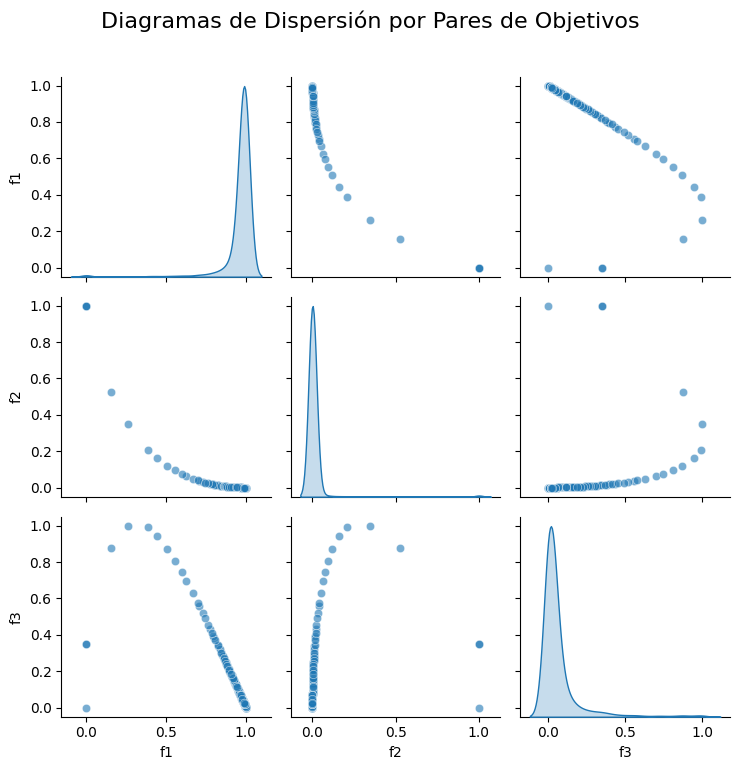
\includegraphics[width=0.9\textwidth]{Images/pareto_projection_moead.png}
    \caption{Proyecciones en 2D entre los objetivos \( f_1 \), \( f_2 \) y \( f_3 \) para MOEA/D. Las distribuciones marginales están en la diagonal principal, mientras que las relaciones entre pares de objetivos se muestran en las subgráficas.}
    \label{fig:objective_projections_moead}
\end{figure}

\textbf{Observaciones clave:}
\begin{itemize}
    \item La relación entre \(f_2\) (regularización) y \(f_3\) (penalización de negatividad) muestra una fuerte correlación no lineal, indicando una interacción más controlada entre estos objetivos.
    \item A diferencia de NSGA-II, \(f_1\) (residual) presenta una tendencia más estructurada en relación con \(f_2\), sugiriendo que MOEA/D logra una asignación más equilibrada en el frente de Pareto.
    \item Las distribuciones marginales son más uniformes en comparación con NSGA-II, lo que refleja el enfoque de descomposición de MOEA/D para generar soluciones equidistantes en el espacio objetivo.
\end{itemize}

\subsection{Comparación entre NSGA-II y MOEA/D}

El análisis de las proyecciones de los objetivos para NSGA-II (Figura \ref{fig:objective_projections_nsga2}) y MOEA/D (Figura \ref{fig:objective_projections_moead}) revela diferencias significativas en cómo estos algoritmos exploran el espacio de soluciones:
\begin{itemize}
    \item NSGA-II tiende a priorizar la diversidad en regiones dominadas por \(f_1\), mientras que MOEA/D genera frentes más uniformes con una mejor representación de \(f_2\) y \(f_3\).
    \item MOEA/D presenta una estructura más definida entre los objetivos, lo que puede ser ventajoso para problemas que requieren soluciones equitativas en el frente.
    \item En aplicaciones donde la positividad y la estabilidad son críticas, MOEA/D muestra un mejor desempeño debido a su habilidad para equilibrar \(f_3\) (penalización de negatividad).
\end{itemize}



%%%%% -------- Analysis -------- %%%%%
\maincontent{Análisis de los Resultados}
\section{Análisis de los Resultados} \label{sec:analysis}

\subsection{Interpretación del Frente de Pareto} \label{sec:analysis:pareto}
El frente de Pareto generado por NSGA-II proporciona una visualización de los compromisos entre fidelidad, regularización y positividad de las soluciones. En particular:
\begin{itemize}
    \item Las soluciones cercanas a la esquina inferior izquierda representan configuraciones donde la fidelidad y la regularización están equilibradas, pero podrían comprometer la positividad.
    \item Las soluciones en la parte superior derecha indican regularización excesiva, lo que resulta en pérdida de fidelidad.
\end{itemize}

El análisis de las distribuciones en el frente de Pareto revela que el uso de NSGA-II permite explorar un rango más amplio de soluciones en comparación con la curva L, que se limita a una única solución.

\subsection{Correlaciones entre Objetivos} \label{sec:analysis:correlations}
La correlación entre los objetivos revela cómo interactúan los compromisos entre fidelidad (\( f_1 \)), regularización (\( f_2 \)) y positividad (\( f_3 \)). La matriz de correlación (Figura \ref{fig:correlation_matrix}) destaca:
\begin{itemize}
    \item Una fuerte correlación negativa entre \( f_1 \) y \( f_3 \), lo que sugiere que las soluciones con menor negatividad tienden a tener menor fidelidad.
    \item Una correlación positiva entre \( f_2 \) y \( f_3 \), indicando que soluciones con mayor regularización también mejoran la positividad, aunque con una posible penalización en fidelidad.
\end{itemize}

Estos resultados proporcionan una base para priorizar objetivos dependiendo de los requisitos de la aplicación.

\subsection{Impacto del Nivel de Ruido} \label{sec:analysis:noise}
El nivel de ruido afecta significativamente el desempeño de NSGA-II. Como se observa en la Figura \ref{fig:pareto_noise}, niveles más altos de ruido desplazan el frente de Pareto hacia soluciones menos precisas, destacando:
\begin{itemize}
    \item NSGA-II mantiene su capacidad para generar soluciones robustas frente a niveles moderados de ruido (\( \sigma = 0.05 \)).
    \item La curva L, en comparación, es más sensible al ruido, lo que puede limitar su utilidad en escenarios altamente ruidosos.
\end{itemize}

\subsection{Comparación con la Curva L} \label{sec:analysis:lcurve}
Aunque la curva L proporciona una solución directa y computacionalmente eficiente, los resultados muestran que NSGA-II ofrece:
\begin{itemize}
    \item Soluciones adaptables a múltiples objetivos y restricciones.
    \item Mejor manejo de restricciones físicas, como la positividad.
    \item Flexibilidad para analizar la sensibilidad del problema al variar el nivel de ruido.
\end{itemize}

Esto sugiere que NSGA-II no solo complementa, sino que puede superar las limitaciones del enfoque basado únicamente en la curva L.

\subsection{Conclusiones del Análisis} \label{sec:analysis:conclusions}
Este análisis destaca la eficacia de NSGA-II para abordar problemas de regularización en la reconstrucción de imágenes fotoacústicas. En comparación con la curva L, NSGA-II:
\begin{itemize}
    \item Proporciona una herramienta poderosa para explorar un rango más amplio de soluciones.
    \item Incorpora objetivos adicionales que mejoran la calidad física y matemática de las soluciones.
    \item Permite una mayor adaptabilidad a condiciones experimentales, como el ruido y las restricciones específicas de la aplicación.
\end{itemize}

Futuras investigaciones podrían enfocarse en optimizar la selección de objetivos y analizar la robustez del enfoque para escenarios más complejos y dimensionalidades mayores.


%%%%% ------ Paper 4 ------ %%%%%
% \maincontent{Congratulations, Doctor.}
% \sectionnote{Here I could write something to provide some meta-information for an annual review, if I wanted to.}


\section{Explanation of the text}

The chapter provides an exegesis for the fourth paper included in this research: good work.

\subsection{Motivation}
The fourth part of this research concerns...





% %%%%% ------ Paper 5 ------ %%%%%
% \maincontent{Okay, nobody likes a show-off}
% \sectionnote{Here I could write something to provide some meta-information for an annual review, if I wanted to.}


\section{Explanation of the text}

The chapter provides an exegesis for the fifth paper included in this research: something really useful, I'm sure. 

\subsection{Motivation}
The fifth part of this research involves...



%%%%% ------ Conclusion ------ %%%%%
\maincontent{Conclusiones}
Este estudio exploró el uso de optimización multiobjetivo mediante los algoritmos NSGA-II y MOEA/D para abordar los desafíos de regularización en la reconstrucción de imágenes fotoacústicas. Los resultados obtenidos demuestran que ambos algoritmos son herramientas poderosas que superan las limitaciones del método tradicional de la curva L. 

NSGA-II destacó por su capacidad para generar soluciones diversas, particularmente en regiones donde la fidelidad (\( f_1 \)) es prioritaria, mientras que MOEA/D mostró un mejor equilibrio en la exploración del frente de Pareto. Ambos algoritmos permitieron analizar los compromisos entre fidelidad, regularización y positividad, proporcionando una base sólida para seleccionar soluciones adaptadas a las restricciones específicas del problema.

Además, los análisis de correlaciones y proyecciones en 2D mostraron cómo interactúan los objetivos, proporcionando una mejor comprensión de las dependencias entre ellos. Esto resulta crucial para guiar futuras aplicaciones en escenarios experimentales realistas, donde el ruido y otras limitaciones físicas son factores determinantes.

En general, este trabajo sienta las bases para futuras investigaciones en la optimización de hiperparámetros y la extensión de los métodos de reconstrucción a dimensiones más altas, como en imágenes 2D y 3D. Estos avances permitirán desarrollar herramientas más robustas y adaptables para aplicaciones biomédicas y científicas.

%%%%% ------ References ------ %%%%%
%\backmatter{Referencias}
\bibliographystyle{plain}
\bibliography{references}

\end{document}